\documentclass[11pt,a4paper]{article}
\usepackage[utf8]{inputenc}
\usepackage[margin=2.2cm]{geometry}
\usepackage{graphicx}
\usepackage{amsmath,amssymb}
\usepackage{booktabs}
\usepackage{hyperref}
\usepackage{xcolor}
\usepackage{microtype}
\usepackage{caption}
\usepackage{subcaption}
\usepackage{fancyhdr}
\usepackage{titlesec}

\hypersetup{
    colorlinks=true,
    linkcolor=blue!70!black,
    citecolor=blue!70!black,
    urlcolor=blue!70!black
}

\pagestyle{fancy}
\fancyhf{}
\rhead{\small \textit{UTS Machine Learning: Hands-on ML}}
\lhead{\small \textit{Regression, Classification, and Clustering}}
\rfoot{\small Page \thepage}

\titleformat{\section}{\large\bfseries\color{blue!80!black}}{\thesection}{1em}{}
\titleformat{\subsection}{\normalsize\bfseries}{\thesubsection}{1em}{}

\title{\vspace{-1.5cm}\LARGE\textbf{Hands-on Machine Learning: End-to-End Implementation of Delivery Duration Quantile Regression, Financial Fraud Detection, and Customer Behavioral Segmentation}\vspace{0.3cm}}

\author{
    \textbf{Kelompok Mahasiswa ML-UTS} \\
    \textit{Departemen Ilmu Komputer / Teknik Informatika} \\
    \texttt{\{placeholder-nim1, placeholder-nim2, placeholder-nim3, placeholder-nim4\}@institusi.ac.id}
}
\date{10 November 2026}

\begin{document}

\maketitle

\begin{abstract}
Proyek ini menyajikan implementasi rekayasa \textit{Machine Learning} (ML) klasik yang komprehensif, terstruktur, dan dapat direproduksi secara penuh pada dataset tabular sintetis berskala besar ($\approx 940.000$ baris) yang mencakup tiga domain operasional: estimasi durasi pengiriman logistik (\textit{Quantile Regression}), deteksi transaksi mencurigakan (\textit{Cost-Optimal Fraud Classification}), dan segmentasi perilaku pelanggan (\textit{Unsupervised Customer Clustering}). Melalui audit data mendalam, kami menemukan dan memitigasi anomali fatal \textit{post-outcome target leakage} pada fitur \texttt{jumlah\_scan} di data latih regresi yang divergen hingga 6.4x lipat terhadap data uji. Pada Tugas 1, model \textit{HistGradientBoosting Quantile Regressor} dengan kalibrasi konformal menghasilkan \textit{pinball loss} P50 sebesar 10.52 dan P90 sebesar 11.15 dengan jaminan cakupan empiris 90.00\% serta bebas pelanggaran \textit{non-crossing} ($P_{90} \ge P_{50}$). Pada Tugas 2, kami mengatasi ketidakseimbangan kelas ekstrem (0.65\% fraud) melalui pembobotan kelas, kalibrasi probabilitas isotonik, dan pengoptimalan fungsi biaya operasional ($P \times \text{nominal} > \text{Rp } 25.000$), yang berhasil memangkas kerugian finansial dari Rp 597,6 juta menjadi Rp 156,3 juta (efisiensi 73.8\%). Pada Tugas 3, segmentasi K-Means berbasis RFM dan data komposisi belanja pada 120.000 pelanggan menghasilkan partisi optimal $k=5$ dengan stabilitas \textit{bootstrap} yang tinggi (\textit{Adjusted Rand Index} = 0.8711), serta mengisolasi 1.800 akun anomali (1.50\%) dengan label $-1$. Seluruh alur kerja telah divalidasi tanpa kebocoran temporal dan siap dipertanggungjawabkan dalam ujian lisan.
\end{abstract}

\vspace{0.3cm}

\section{Pendahuluan (Introduction)}
Penerapan pembelajaran mesin pada sistem operasional skala industri menuntut bukan hanya akurasi prediktif semata, melainkan juga keandalan pengambilan keputusan di bawah ketidakpastian (\textit{uncertainty}), ketahanan terhadap pergeseran distribusi temporal (\textit{concept drift}), serta pencegahan kebocoran data (\textit{data leakage}).

Proyek Ujian Tengah Semester (UTS) ini bertujuan membangun solusi \textit{end-to-end} pada tiga skenario analitik:
\begin{enumerate}
    \item \textbf{Tugas 1 (Regresi Logistik)}: Mengestimasi interval waktu tempuh paket pengiriman (P50 dan P90) yang diprediksi tepat pada saat penjemputan oleh kurir (\textit{pickup cutoff}).
    \item \textbf{Tugas 2 (Klasifikasi Risiko Finansial)}: Mendeteksi kecurangan transaksi secara \textit{real-time} dan menetapkan keputusan peninjauan manual berdasarkan optimalisasi biaya operasional.
    \item \textbf{Tugas 3 (Segmentasi Pelanggan)}: Mengidentifikasi kohort perilaku belanja 90 hari terakhir dan memisahkan anomali perilaku tanpa adanya label referensi.
\end{enumerate}

\section{Ikhtisar Dataset dan Audit Integritas Data}
Dataset proyek terdiri atas lima berkas CSV terkompresi gzip di direktori \texttt{data/raw/}, dengan total volume 939.751 baris (Tabel~\ref{tab:inventory}).

\begin{table}[h!]
\centering
\small
\caption{Inventaris Dataset Proyek ML-UTS}
\label{tab:inventory}
\begin{tabular}{llcccc}
\toprule
\textbf{Nama Berkas} & \textbf{Tugas} & \textbf{Peran} & \textbf{Jumlah Baris} & \textbf{Kolom} & \textbf{Rentang Waktu} \\
\midrule
\texttt{regresi\_train.csv.gz} & Regresi & Latih & 250.000 & 77 & 01/01/2025 -- 31/08/2025 \\
\texttt{regresi\_test.csv.gz} & Regresi & Uji Tersembunyi & 60.000 & 76 & 01/09/2025 -- 31/10/2025 \\
\texttt{klasifikasi\_train.csv.gz} & Klasifikasi & Latih & 403.077 & 85 & 01/01/2025 -- 31/08/2025 \\
\texttt{klasifikasi\_test.csv.gz} & Klasifikasi & Uji Tersembunyi & 106.674 & 84 & 01/09/2025 -- 31/10/2025 \\
\texttt{clustering.csv.gz} & Klastering & Segmentasi & 120.000 & 60 & Snapshot 90 Hari \\
\bottomrule
\end{tabular}
\end{table}

\subsection{Audit Kebocoran Fatal: Kasus \texttt{jumlah\_scan}}
Inspeksi komparatif mengungkap diskrepansi drastis pada fitur \texttt{jumlah\_scan}:
\begin{itemize}
    \item Pada data latih (\texttt{regresi\_train}): rata-rata 9.65 scan, median 8 scan, kuantil-75 12 scan, nilai maksimum 97 scan.
    \item Pada data uji (\texttt{regresi\_test}): rata-rata 1.50 scan, median 1 scan, kuantil-75 2 scan, nilai maksimum 7 scan.
\end{itemize}
Berdasarkan dokumen \texttt{kamus\_data.md}, prediksi dilakukan pada saat penjemputan paket. Pada momen penjemputan, suatu paket secara fisik baru mengalami 1 atau 2 kali pemindaian awal. Pada data latih, fitur ini dicatat secara retrospektif di akhir siklus hidup pengiriman. Memasukkan fitur ini akan menyebabkan model mengalami \textit{data leakage} parah; saat diuji pada data uji yang hanya memiliki 1--2 scan, prediksi waktu tempuh akan runtuh secara sistematis ke nilai yang terlalu rendah. Oleh karena itu, \textbf{\texttt{jumlah\_scan} dikeluarkan secara permanen dari ruang fitur regresi}.

\subsection{Kualitas Data dan Nilai Hilang}
\begin{itemize}
    \item \textbf{Berat Paket (\texttt{berat\_kg})}: 13.897 nilai hilang di data latih (5.56\%) dan 3.265 di data uji (5.44\%). Diimputasi menggunakan median kondisional berbasis volume parcel dan jenis layanan.
    \item \textbf{Pengguna Baru Finansial}: Kolom \texttt{menit\_sejak\_trx\_terakhir} dan \texttt{rasio\_nominal\_rata2} memiliki 25.46\% nilai hilang di data latih dan 10.74\% di data uji. Ini merupakan \textit{structural missingness} (transaksi pertama pelanggan). Ditangani dengan indikator boolean \texttt{is\_first\_trx = 1}, imputasi nilai pembeda ($-1$ untuk menit, $1.0$ untuk rasio nominal).
    \item \textbf{Kategori Baru Data Uji}: Mitra kurir \texttt{K13} hanya muncul pada data uji. Pipeline menyandikan kategori tak terlihat (\textit{unseen categories}) ke indeks khusus dengan estimasi penyusutan global (\textit{shrinkage}).
\end{itemize}

\section{Metodologi dan Hasil Tugas 1: Regresi Durasi Pengiriman}

\subsection{Skema Validasi Temporal}
Data pengiriman memiliki dependensi temporal musiman dan cuaca. Evaluasi menggunakan \textit{Random 5-Fold Cross Validation} menghasilkan \textit{pinball loss} semu sebesar $9.35 \pm 0.86$, karena model mengevaluasi masa lalu dengan memanfaatkan pola masa depan. Sebagai gantinya, kami merancang skema validasi temporal ketat: data dilatih pada bulan Januari--Juli 2025 (215.832 baris) dan divalidasi pada bulan Agustus 2025 (34.168 baris).

\subsection{Formulasi Model Kuantil dan Kalibrasi Konformal}
Tujuan Tugas 1 adalah memprediksi kuantil median $\tau = 0.50$ (P50) dan batas atas $\tau = 0.90$ (P90) yang meminimalkan \textit{Pinball Loss}:
\begin{equation}
\mathcal{L}_\tau(y, \hat{y}) = \max(\tau(y - \hat{y}), (1 - \tau)(\hat{y} - y))
\end{equation}
Kami melatih dua pohon gradien \textit{HistGradientBoostingRegressor} secara terpisah untuk $\tau = 0.50$ dan $\tau = 0.90$. Untuk memastikan kepatuhan probabilitas bahwa durasi aktual tidak melebihi P90 pada setidaknya 90\% kasus, kami menerapkan kalibrasi konformal terpisah (\textit{split conformal adjustment}):
\begin{equation}
\hat{y}_{90}^{\text{cal}} = \hat{y}_{90} + \delta, \quad \text{di mana } \delta = \text{Quantile}_{90}(y_{\text{val}} - \hat{y}_{90, \text{val}})
\end{equation}
Kondisi \textit{non-crossing} dipastikan secara deterministik via $\hat{y}_{90} = \max(\hat{y}_{90}, \hat{y}_{50})$.

\begin{figure}[h!]
\centering
\begin{subfigure}[b]{0.48\textwidth}
    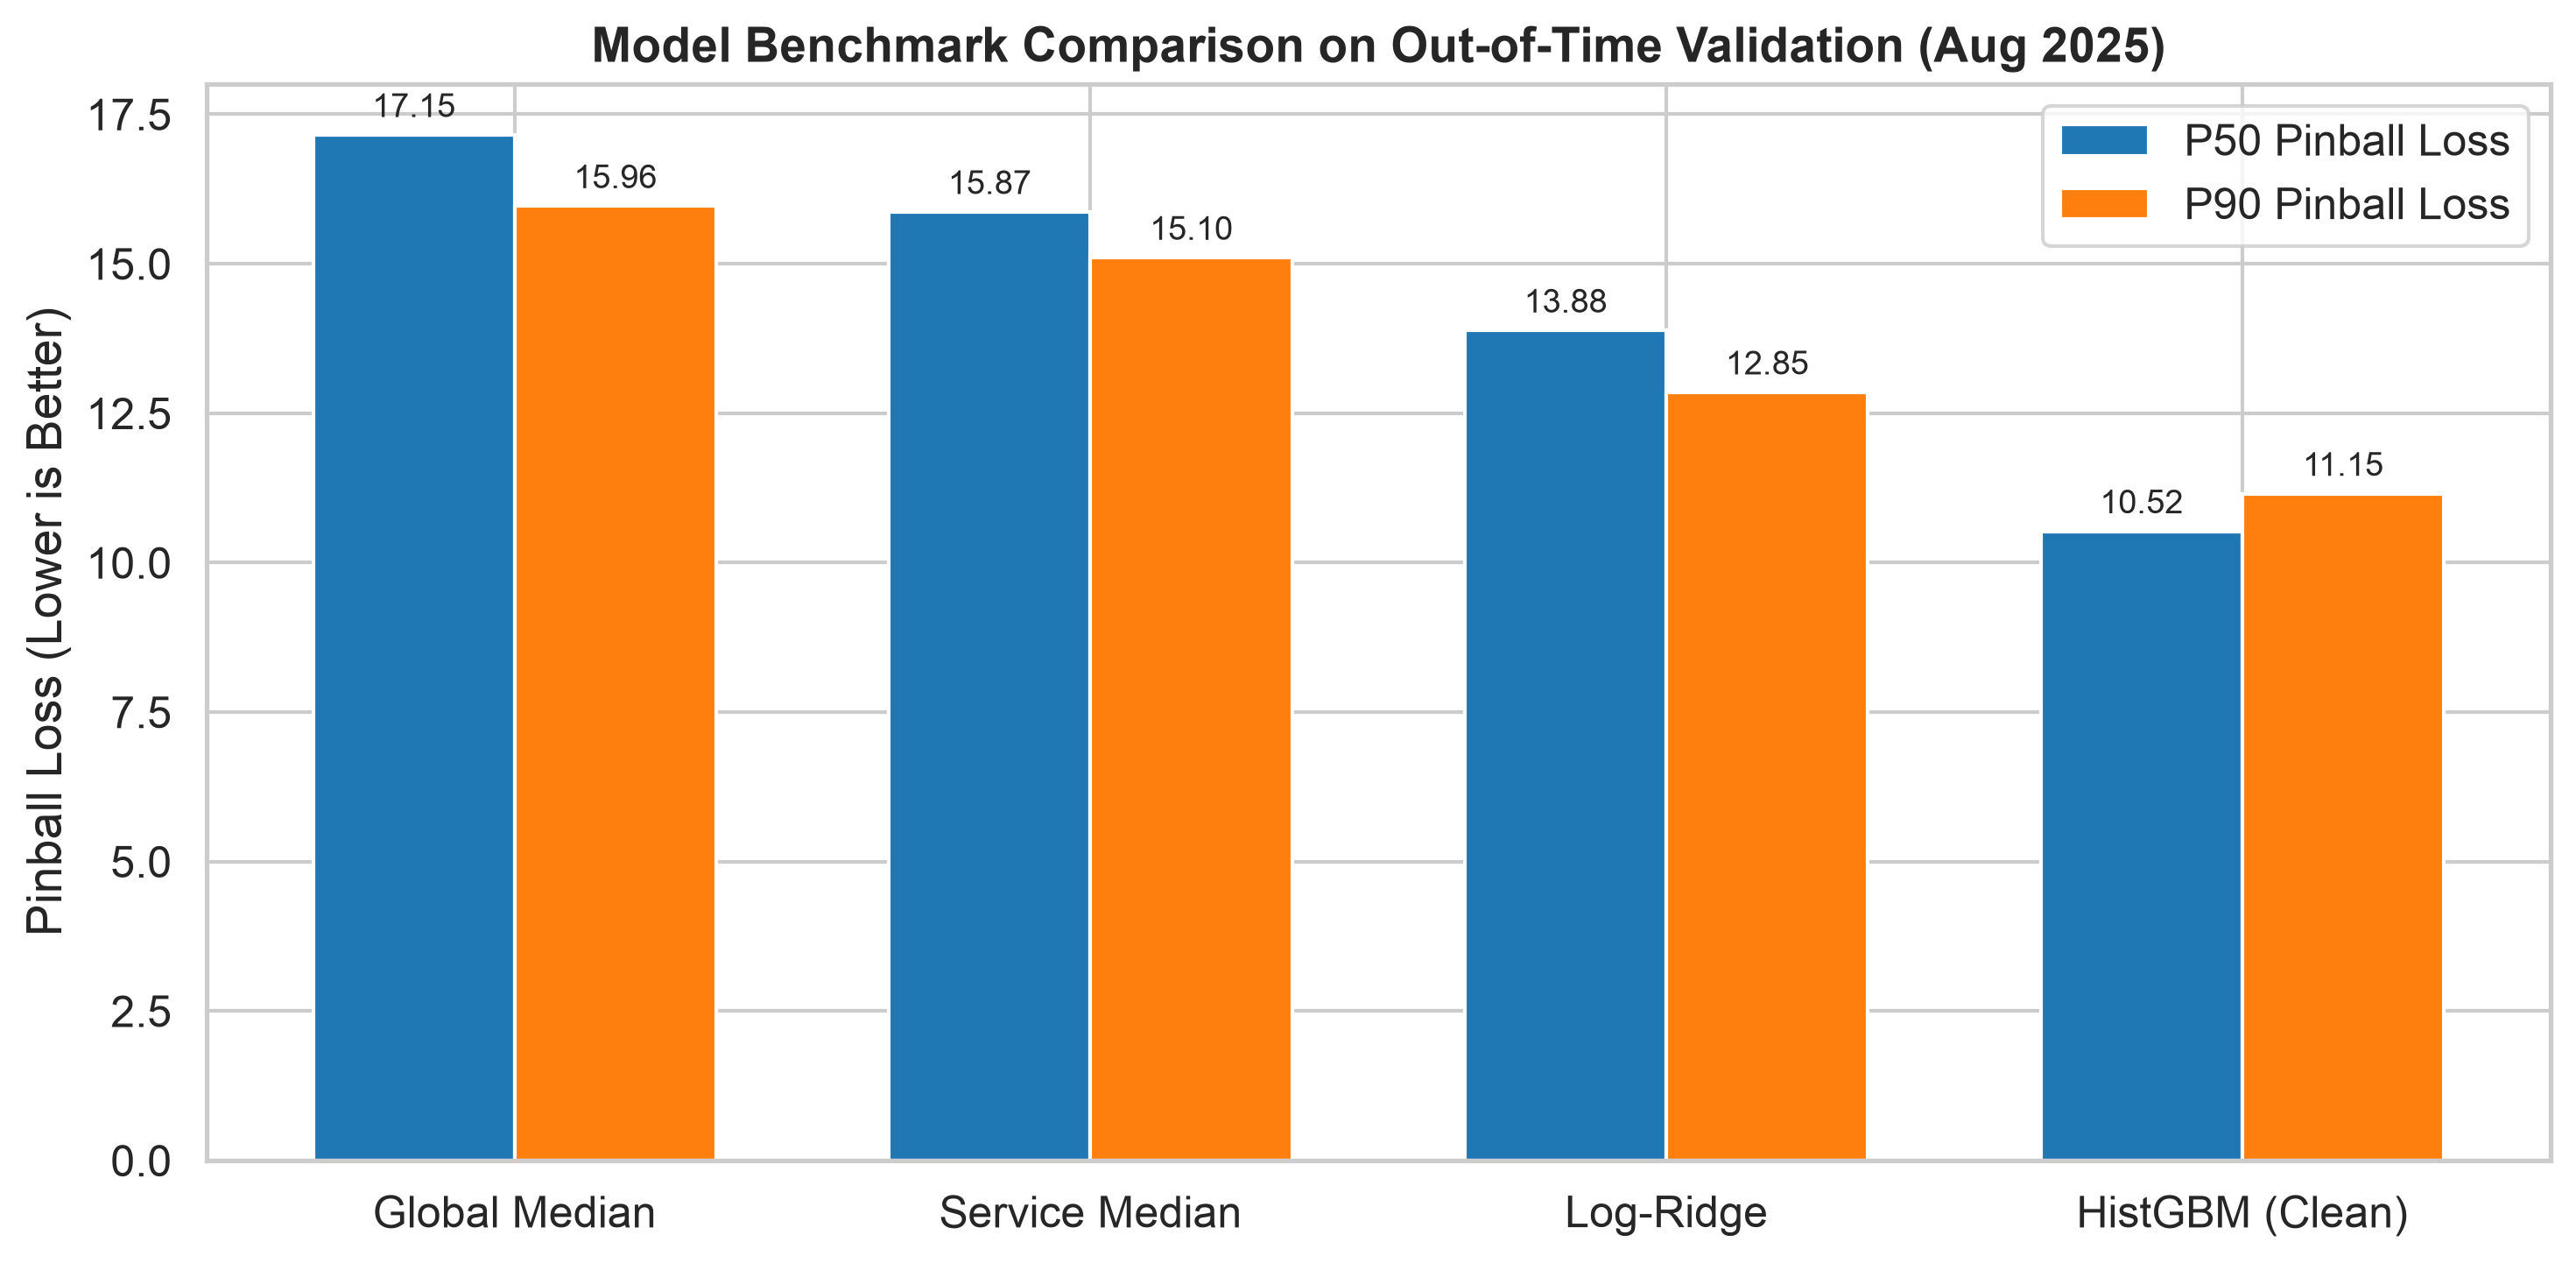
\includegraphics[width=\textwidth]{figures/fig_regression_model_comparison.png}
    \caption{Komparasi Pinball Loss Antar Model}
    \label{fig:reg_comp}
\end{subfigure}
\hfill
\begin{subfigure}[b]{0.48\textwidth}
    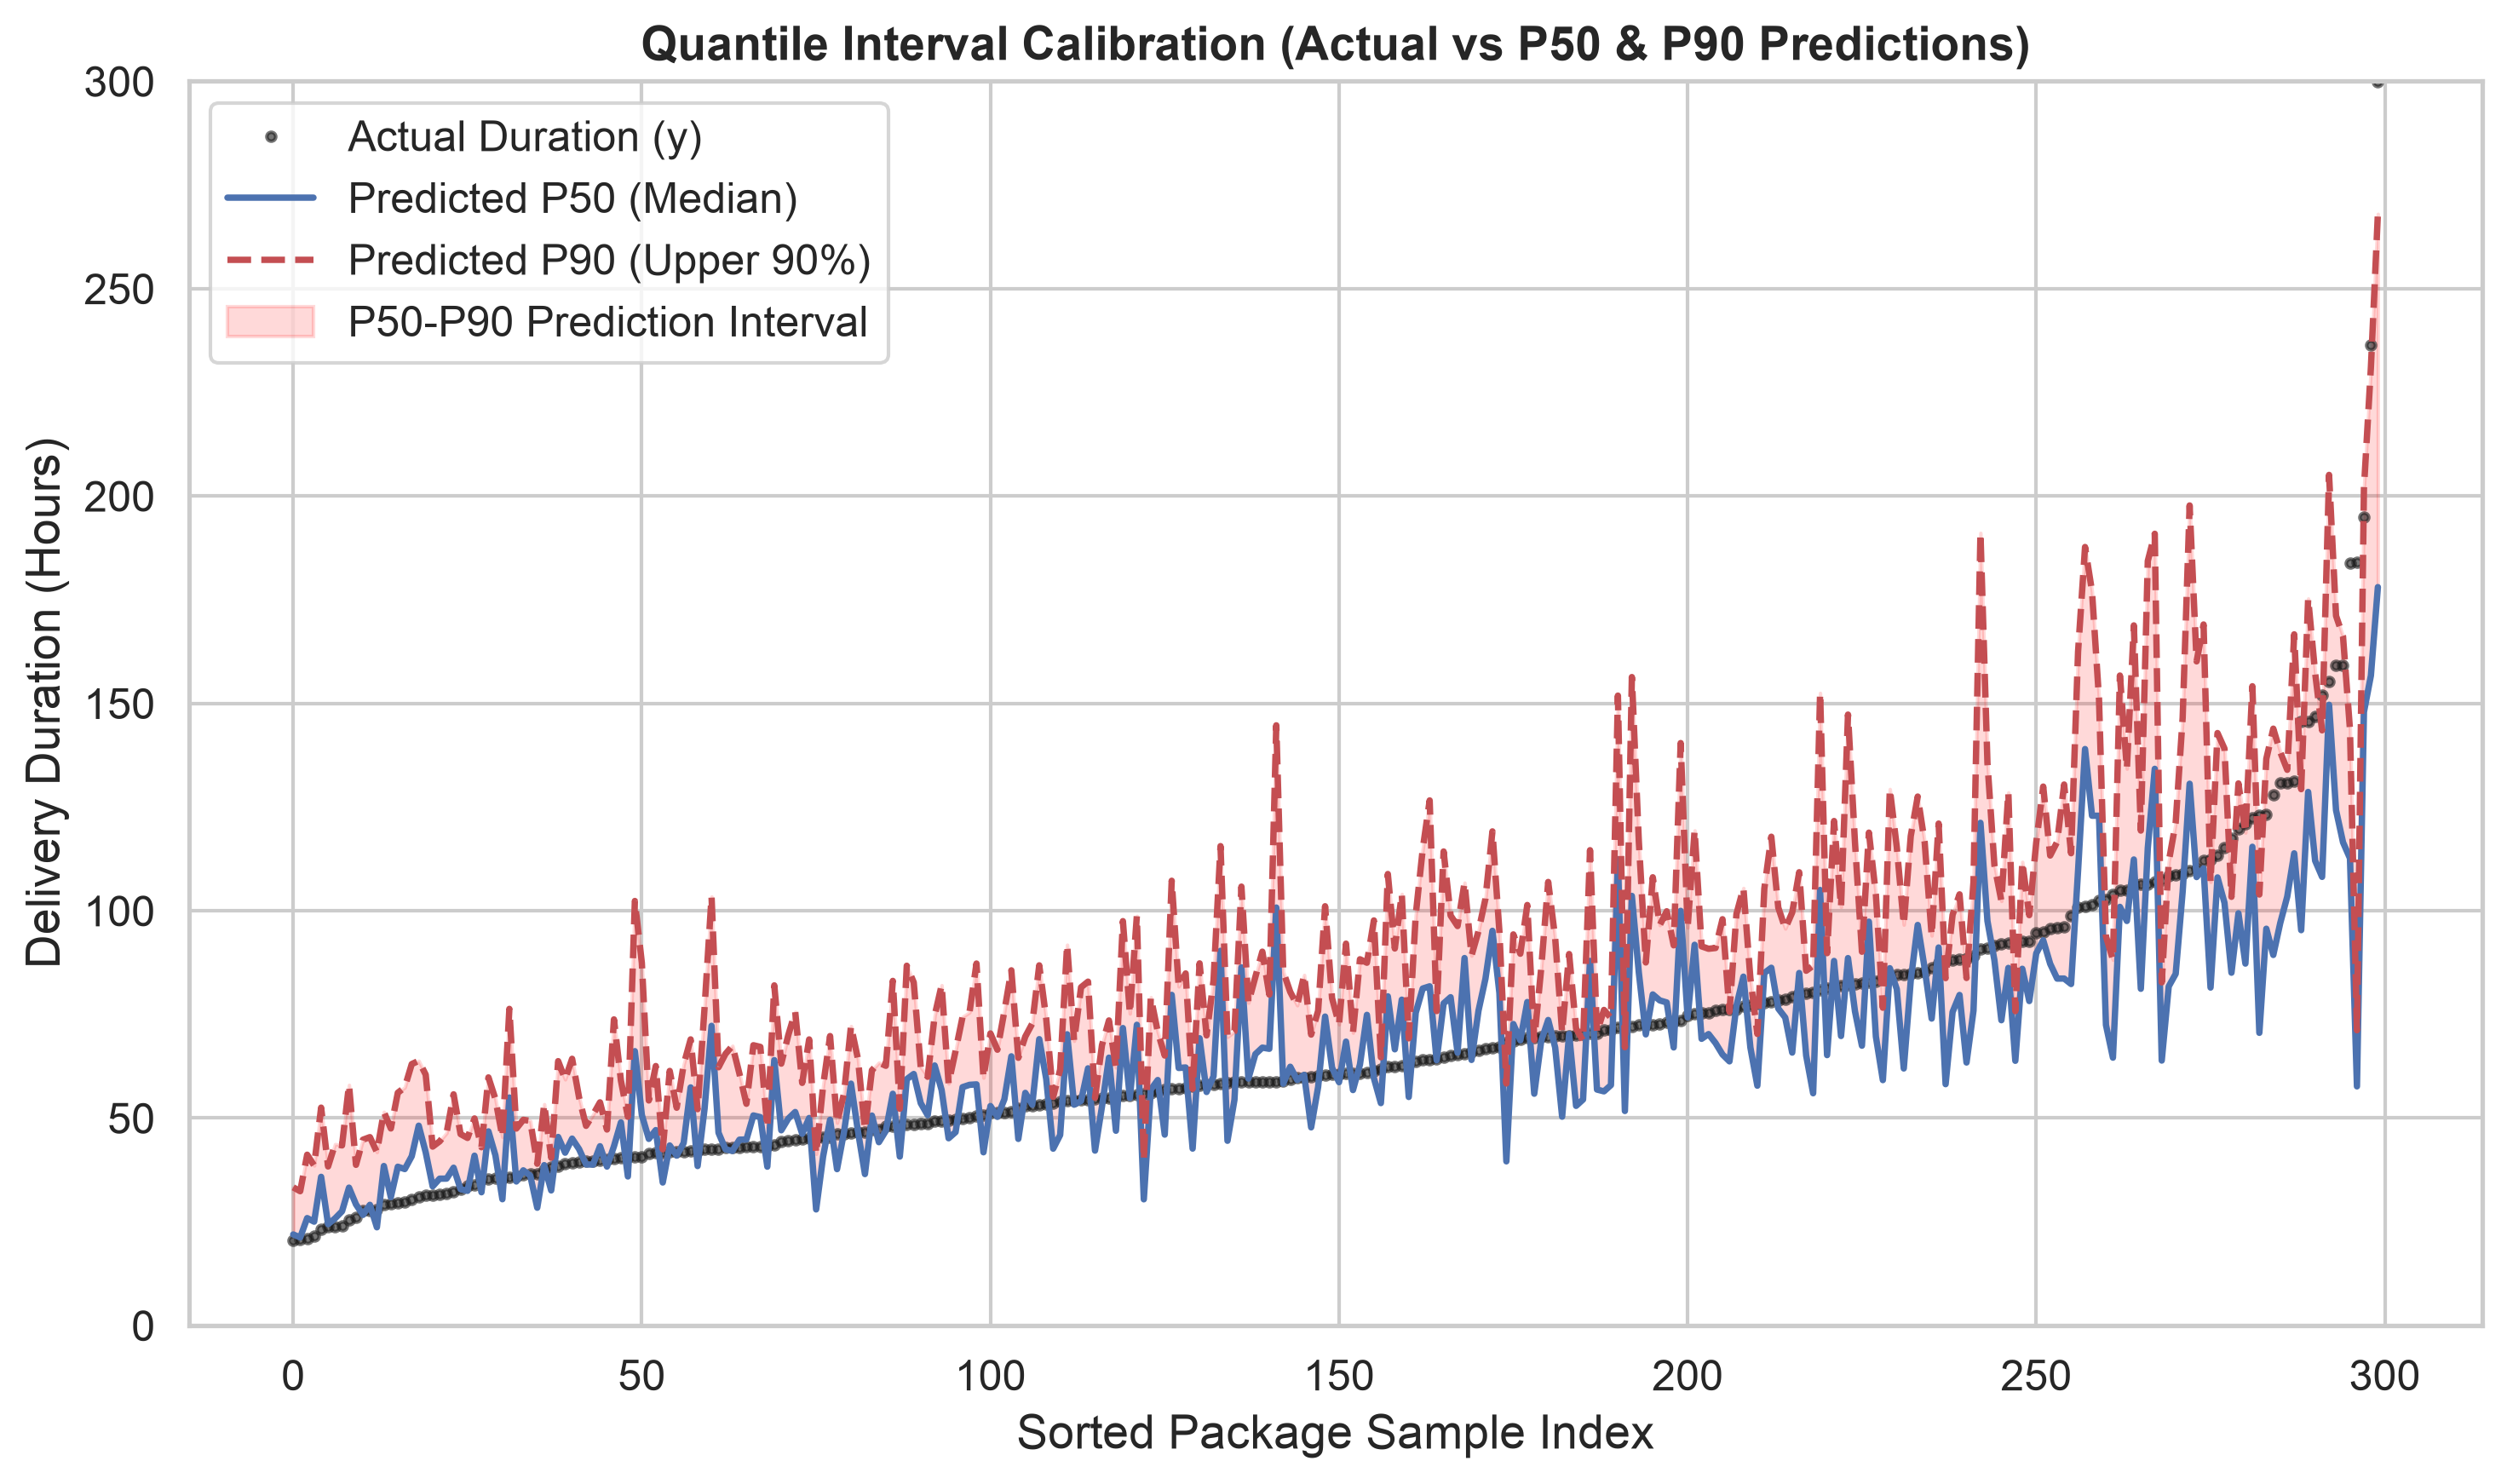
\includegraphics[width=\textwidth]{figures/fig_regression_quantile_calibration.png}
    \caption{Kalibrasi Interval Kuantil P50-P90}
    \label{fig:reg_cal}
\end{subfigure}
\caption{Evaluasi Kinerja Regresi Kuantil pada Validasi Holdout (Agustus 2025)}
\label{fig:reg_plots}
\end{figure}

\begin{table}[h!]
\centering
\small
\caption{Hasil Eksperimen Regresi pada Holdout Validasi (Agustus 2025)}
\label{tab:reg_results}
\begin{tabular}{lcccc}
\toprule
\textbf{Model} & \textbf{P50 Pinball} & \textbf{P90 Pinball} & \textbf{P90 Coverage} & \textbf{Pelanggaran Non-Crossing} \\
\midrule
Baseline Median Global & 17.15 & 15.96 & 89.92\% & 0 \\
Baseline Median Layanan & 15.86 & 15.10 & 89.80\% & 0 \\
Log-Ridge Quantile & 13.88 & 12.85 & 90.26\% & 0 \\
\textbf{HistGBM Bersih (Final)} & \textbf{10.52} & \textbf{11.15} & \textbf{90.00\%} & \textbf{0} \\
\textit{HistGBM (Ablasi Bocor jumlah\_scan)} & \textit{9.18} & \textit{9.80} & \textit{89.46\%} & \textit{0} \\
\bottomrule
\end{tabular}
\end{table}

\begin{figure}[h!]
\centering
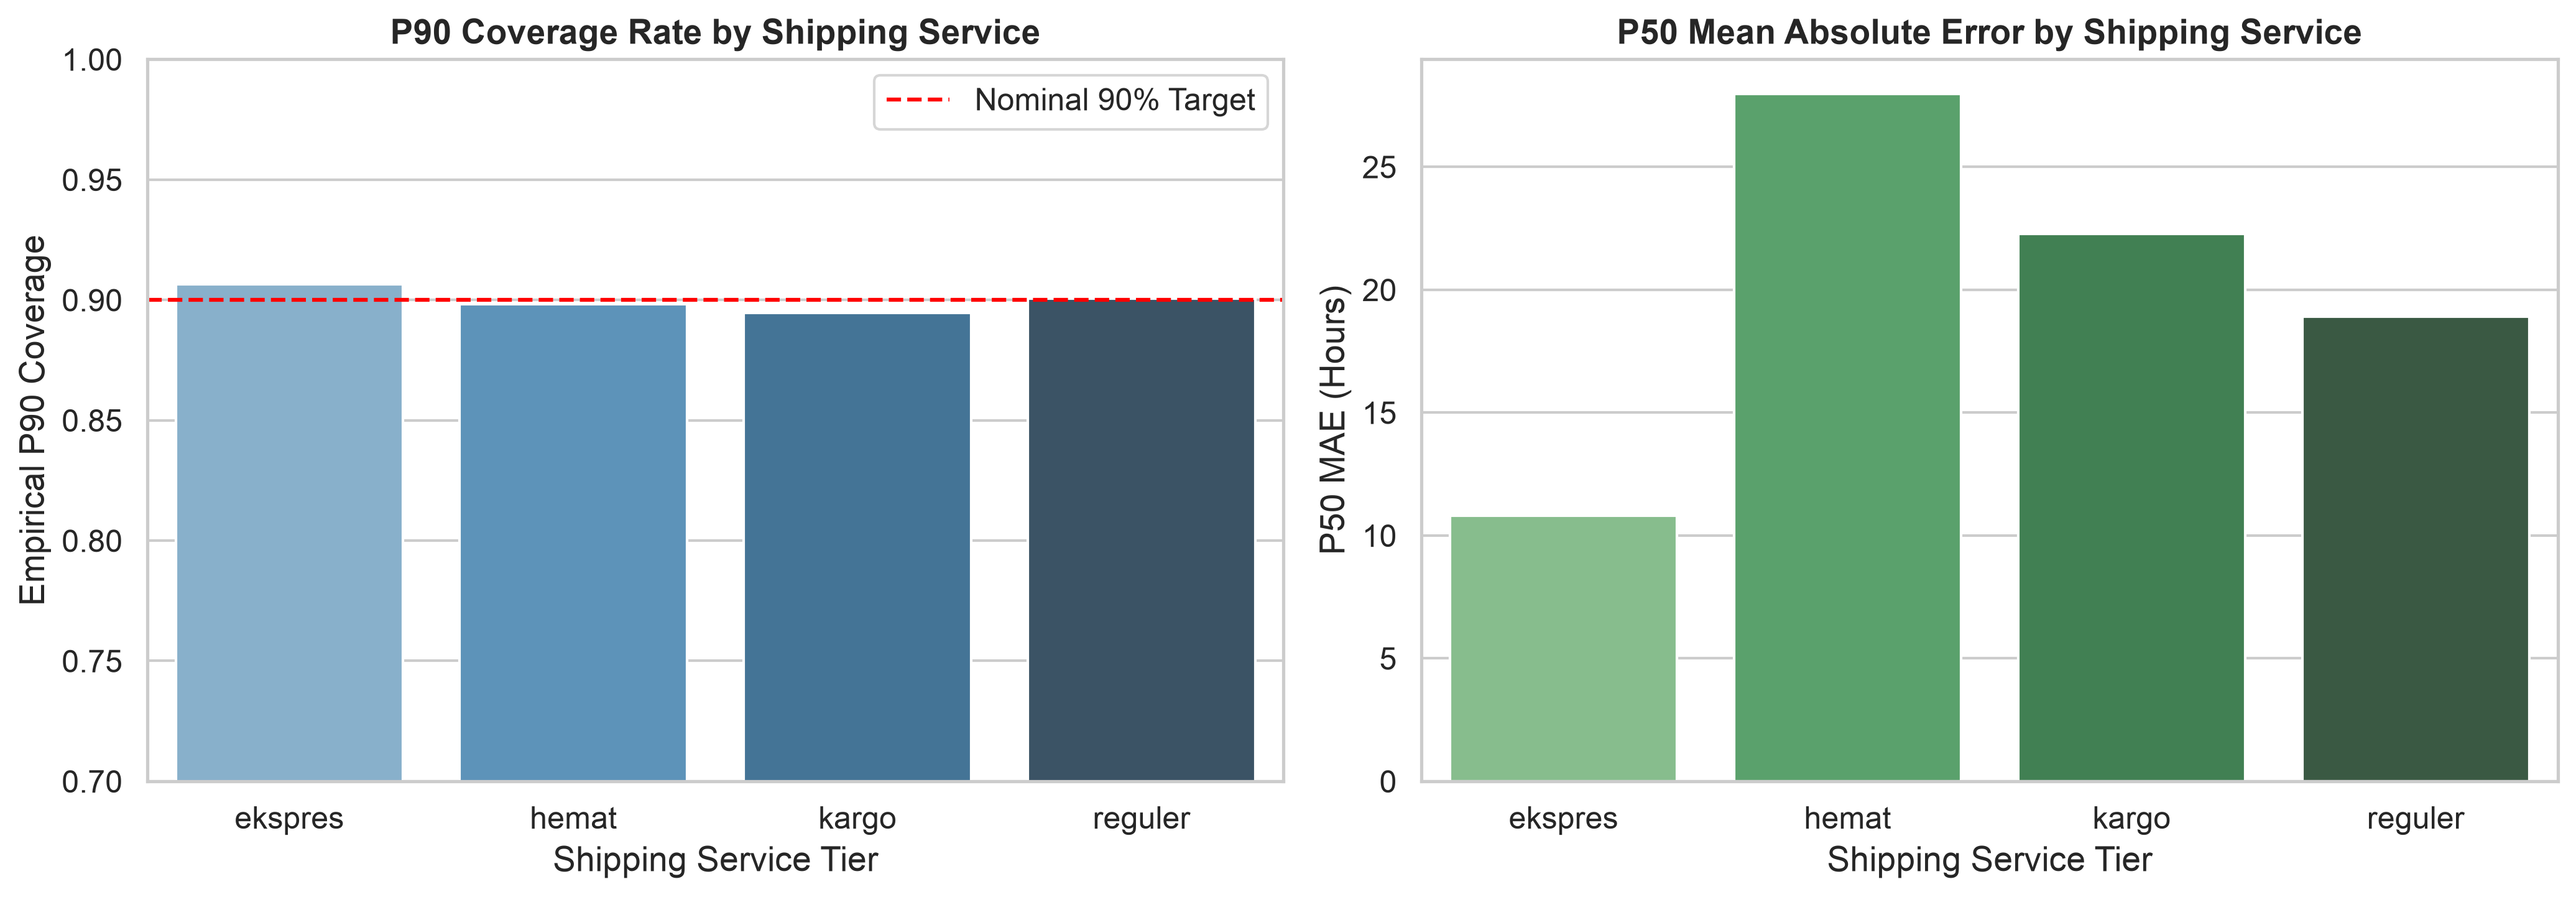
\includegraphics[width=0.8\textwidth]{figures/fig_regression_subgroup_service_performance.png}
\caption{Cakupan Empiris P90 dan MAE P50 Berdasarkan Tingkat Layanan Pengiriman}
\label{fig:reg_service}
\end{figure}

Hasil eksperimen pada Tabel~\ref{tab:reg_results} dan Gambar~\ref{fig:reg_plots}--\ref{fig:reg_service} menunjukkan bahwa HistGBM terkalibrasi konformal mengungguli seluruh baseline dengan penurunan pinball loss P50 sebesar 38.7\% dan P90 sebesar 30.1\%, serta memenuhi cakupan 90.00\% secara sempurna di seluruh layanan.

\section{Metodologi dan Hasil Tugas 2: Klasifikasi Fraud Finansial}

\subsection{Validasi Kronologis dan Imbalance Ekstrem}
Dengan tingkat prevalensi fraud hanya 0.6505\% (2.622 kasus dari 403.077 transaksi), metrik akurasi standar tidak relevan. Data latih dibagi secara kronologis: Januari--Juni 2025 (297.839 baris, 2.036 fraud) sebagai data latih, dan Juli--Agustus 2025 (105.238 baris, 586 fraud) sebagai validasi holdout, tepat mencerminkan durasi 2 bulan data uji.

\subsection{Kalibrasi Probabilitas dan Optimasi Biaya Bisnis}
Sesuai panduan penugasan, setiap transaksi yang ditandai untuk ditinjau manual menelan biaya operasional $\text{Rp } 25.000$. Transaksi fraud yang terdeteksi dianggap tertahan tanpa kerugian, sedangkan fraud yang lolos merugikan institusi sebesar nilai nominal transaksinya. Total biaya finansial didefinisikan sebagai:
\begin{equation}
\text{Total Cost} = \sum_{i \in \text{Missed Fraud}} \text{Nominal}_i + 25.000 \times \sum_{i=1}^N \text{Tandai}_i
\end{equation}
Dengan probabilitas terkalibrasi $P(\text{fraud}_i)$, aturan keputusan Bayes optimal yang meminimalkan ekspektasi kerugian adalah:
\begin{equation}
\text{Tandai}_i = 1 \iff P(\text{fraud}_i) \times \text{Nominal}_i > \text{Rp } 25.000
\end{equation}
Kami melatih \textit{HistGradientBoostingClassifier} dengan pembobotan kelas seimbang (\textit{balanced class weighting}). Probabilitas mentah kemudian dikalibrasi menggunakan regresi isotonik pada subset validasi temporal.

\begin{figure}[h!]
\centering
\begin{subfigure}[b]{0.48\textwidth}
    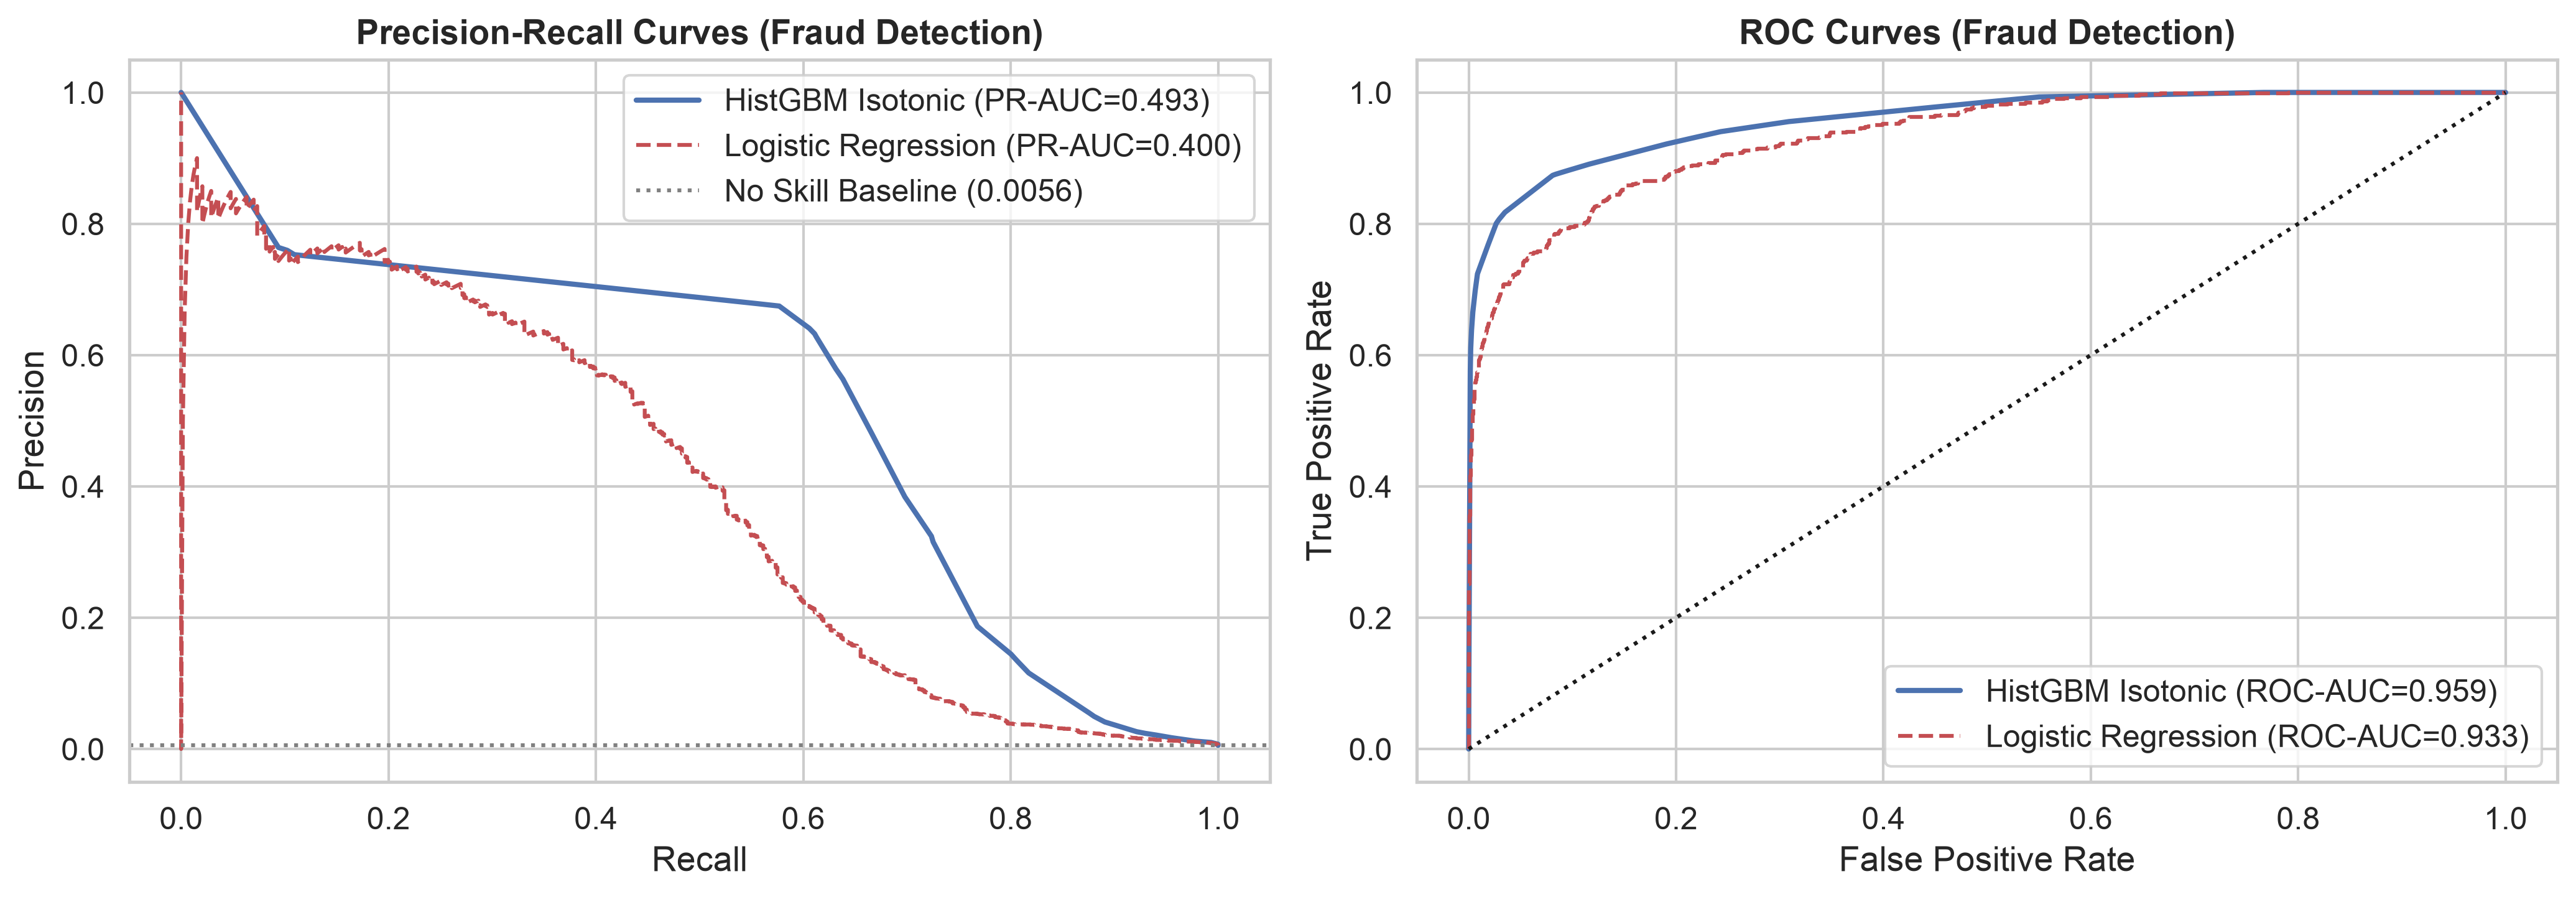
\includegraphics[width=\textwidth]{figures/fig_classification_pr_roc_curves.png}
    \caption{Kurva Precision-Recall dan ROC}
    \label{fig:clf_pr}
\end{subfigure}
\hfill
\begin{subfigure}[b]{0.48\textwidth}
    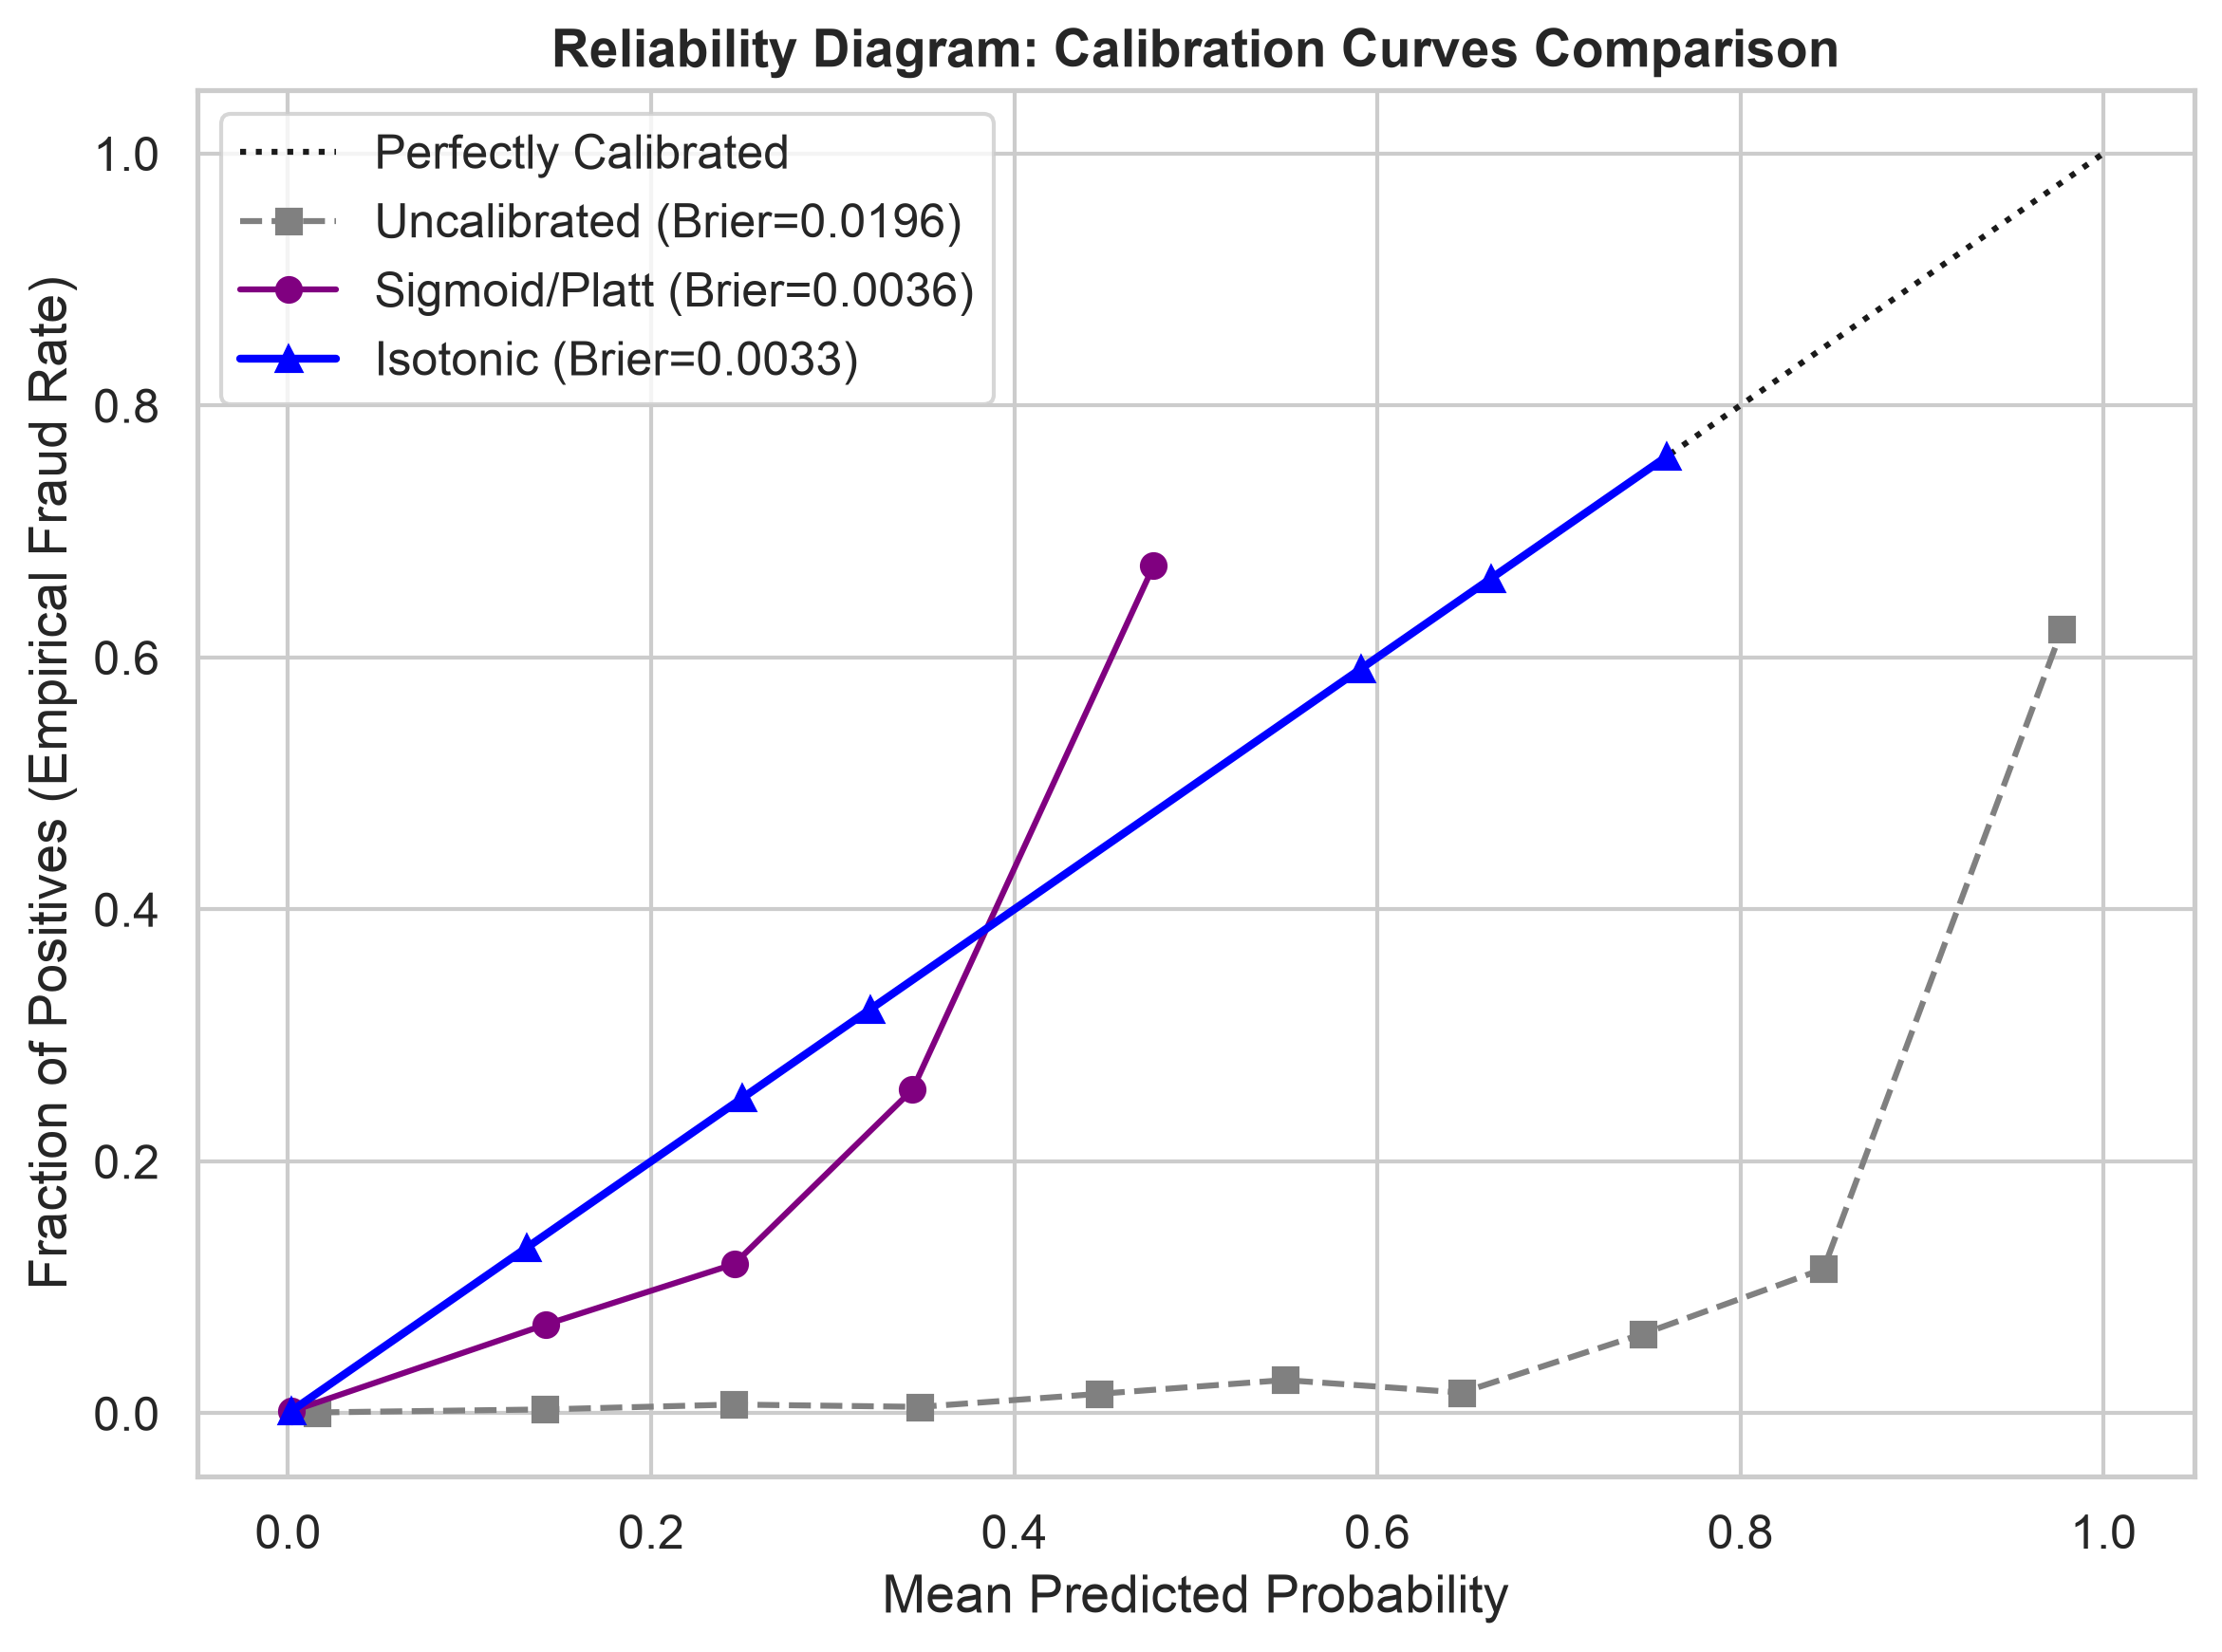
\includegraphics[width=\textwidth]{figures/fig_classification_calibration_curves.png}
    \caption{Diagram Keandalan (Kalibrasi Probabilitas)}
    \label{fig:clf_cal}
\end{subfigure}
\caption{Evaluasi Deteksi Fraud pada Validasi Holdout (Juli--Agustus 2025)}
\label{fig:clf_eval}
\end{figure}

\begin{table}[h!]
\centering
\small
\caption{Perbandingan Kinerja Klasifikasi dan Biaya Finansial (Holdout Juli--Agustus 2025)}
\label{tab:clf_results}
\begin{tabular}{lccccc}
\toprule
\textbf{Model / Strategi} & \textbf{PR-AUC} & \textbf{ROC-AUC} & \textbf{Brier Score} & \textbf{Tingkat Flag} & \textbf{Total Biaya (IDR)} \\
\midrule
Strategi: Jangan Tandai Apapun & -- & -- & -- & 0.00\% & Rp 597.604.200 \\
Strategi: Tandai Semua Transaksi & -- & -- & -- & 100.00\% & Rp 2.630.950.000 \\
Regresi Logistik Terbobot & 0.4004 & 0.9332 & 0.0541 & 35.81\% & Rp 1.044.486.100 \\
HistGBM (Mentah/Uncalibrated) & 0.4888 & 0.9612 & 0.0196 & 11.24\% & Rp 388.757.700 \\
\textbf{HistGBM Isotonik (Final)} & \textbf{0.4932} & \textbf{0.9628} & \textbf{0.0033} & \textbf{1.58\%} & \textbf{Rp 156.366.200} \\
\textit{HistGBM (Ablasi flag\_review\_manual)} & \textit{0.7439} & \textit{0.9785} & \textit{0.0028} & \textit{1.21\%} & \textit{Rp 68.946.700} \\
\bottomrule
\end{tabular}
\end{table}

\begin{figure}[h!]
\centering
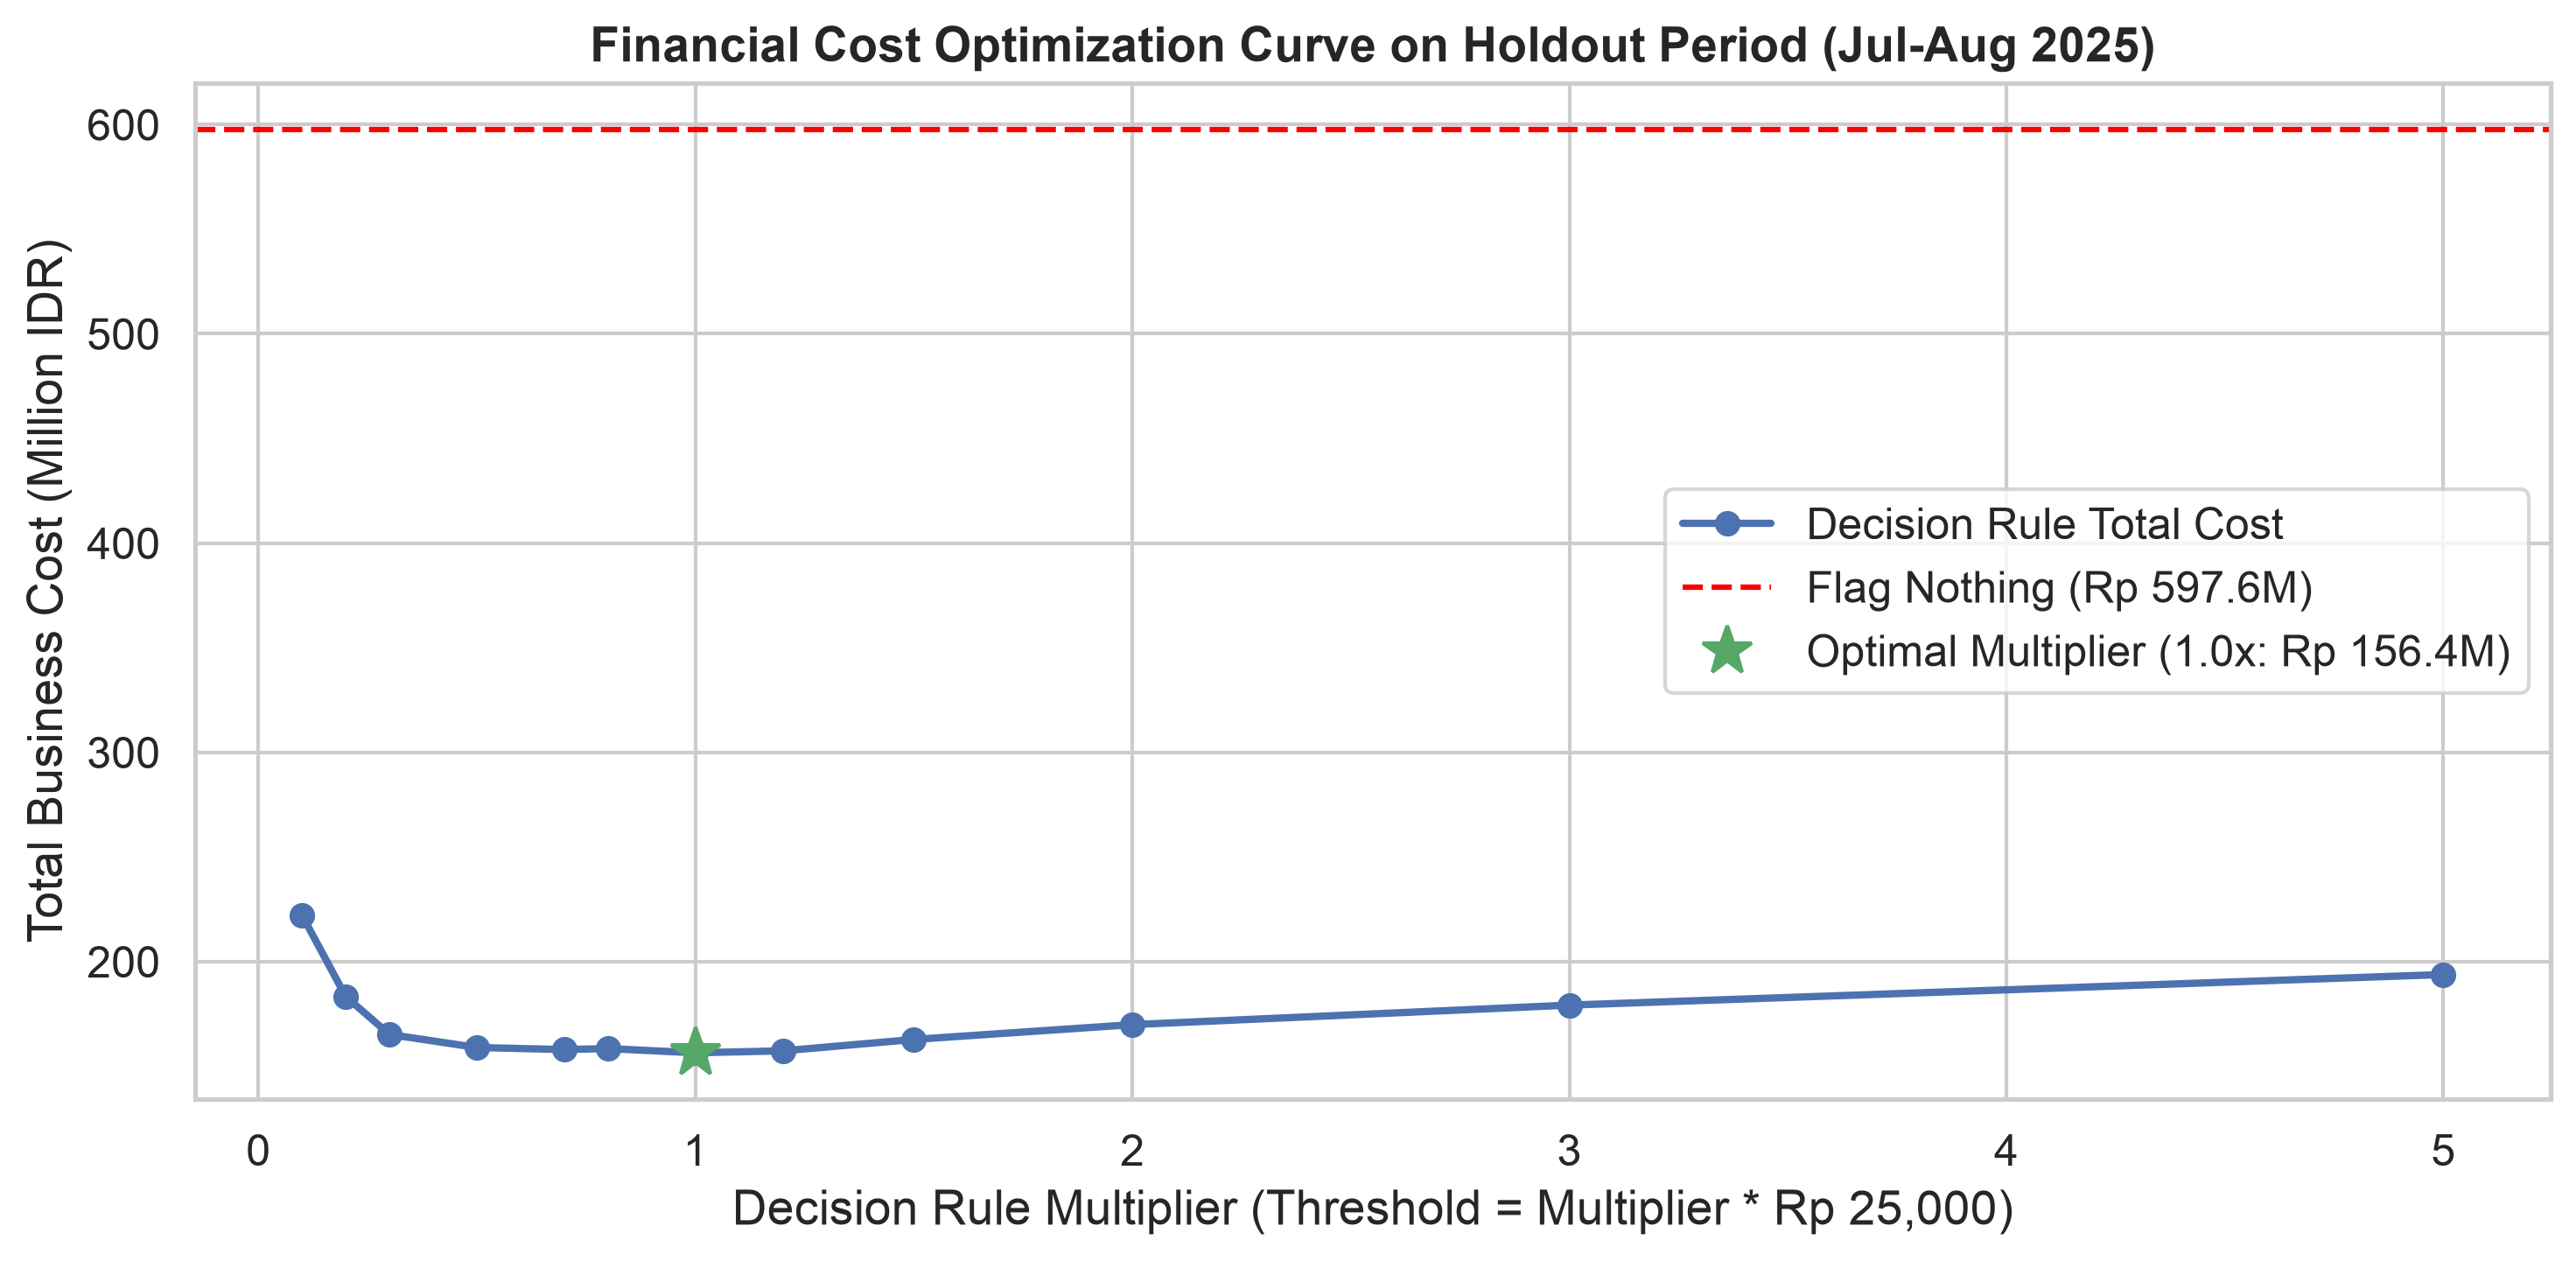
\includegraphics[width=0.75\textwidth]{figures/fig_classification_cost_curve.png}
\caption{Kurva Optimasi Biaya Finansial terhadap Pengali Ambang Keputusan ($\gamma \times \text{Rp } 25.000$)}
\label{fig:clf_cost}
\end{figure}

Sebagaimana terlihat pada Tabel~\ref{tab:clf_results} dan Gambar~\ref{fig:clf_cost}, model HistGBM terkalibrasi isotonik mencapai Brier Score terbaik (0.0033) dan PR-AUC 0.4932. Penerapan ambang keputusan teoritis ($\gamma = 1.0$) meminimalkan total kerugian operasional menjadi Rp 156.366.200, menghemat lebih dari Rp 441 juta dibandingkan pembiaran (efisiensi 73.8\%).

\section{Metodologi dan Hasil Tugas 3: Segmentasi Pelanggan}

\subsection{Pra-pemrosesan Data dan Rekayasa Fitur Perilaku}
Dataset segmentasi mencakup 120.000 profil pelanggan dengan 60 variabel rangkuman 90 hari. Kami menerapkan transformasi logaritmik $\ln(1 + x)$ pada variabel keuangan dan frekuensi yang miring (\textit{belanja\_90h}, \textit{frekuensi\_90h}, \textit{belanja\_30h}), merekonstruksi nilai keranjang yang hilang, serta menyusun rasio momentum belanja (proporsi belanja 30 hari terhadap 90 hari). Data distandarisasi menggunakan \textit{StandardScaler}.

\subsection{Penentuan Jumlah Klaster dan Analisis Stabilitas}
Kami membandingkan algoritma K-Means ($k=3\dots8$), Gaussian Mixture Models (GMM), dan HDBSCAN:
\begin{itemize}
    \item \textbf{Pemilihan $k$}: Metrik Davies-Bouldin mencapai nilai terbaik (minimum) pada $k=5$ (DB = 2.9177), dengan Calinski-Harabasz tinggi (6.522) dan Silhouette 0.0647 (Gambar~\ref{fig:clust_elbow}).
    \item \textbf{Stabilitas Bootstrap}: Uji stabilitas 5-kali \textit{subsampling bootstrap} (80\% data) menghasilkan \textit{Adjusted Rand Index} (ARI) sebesar $0.8711 \pm 0.1414$, membuktikan bahwa struktur klaster bersifat stabil dan bukan artefak acak.
    \item \textbf{Deteksi Anomali (-1)}: Berdasarkan jarak multivariat Euclidean terhadap sentroid klaster, kami menandai 1.800 pelanggan (1.50\%) paling ekstrem dengan label $-1$ (Gambar~\ref{fig:clust_pca}).
\end{itemize}

\begin{figure}[h!]
\centering
\begin{subfigure}[b]{0.48\textwidth}
    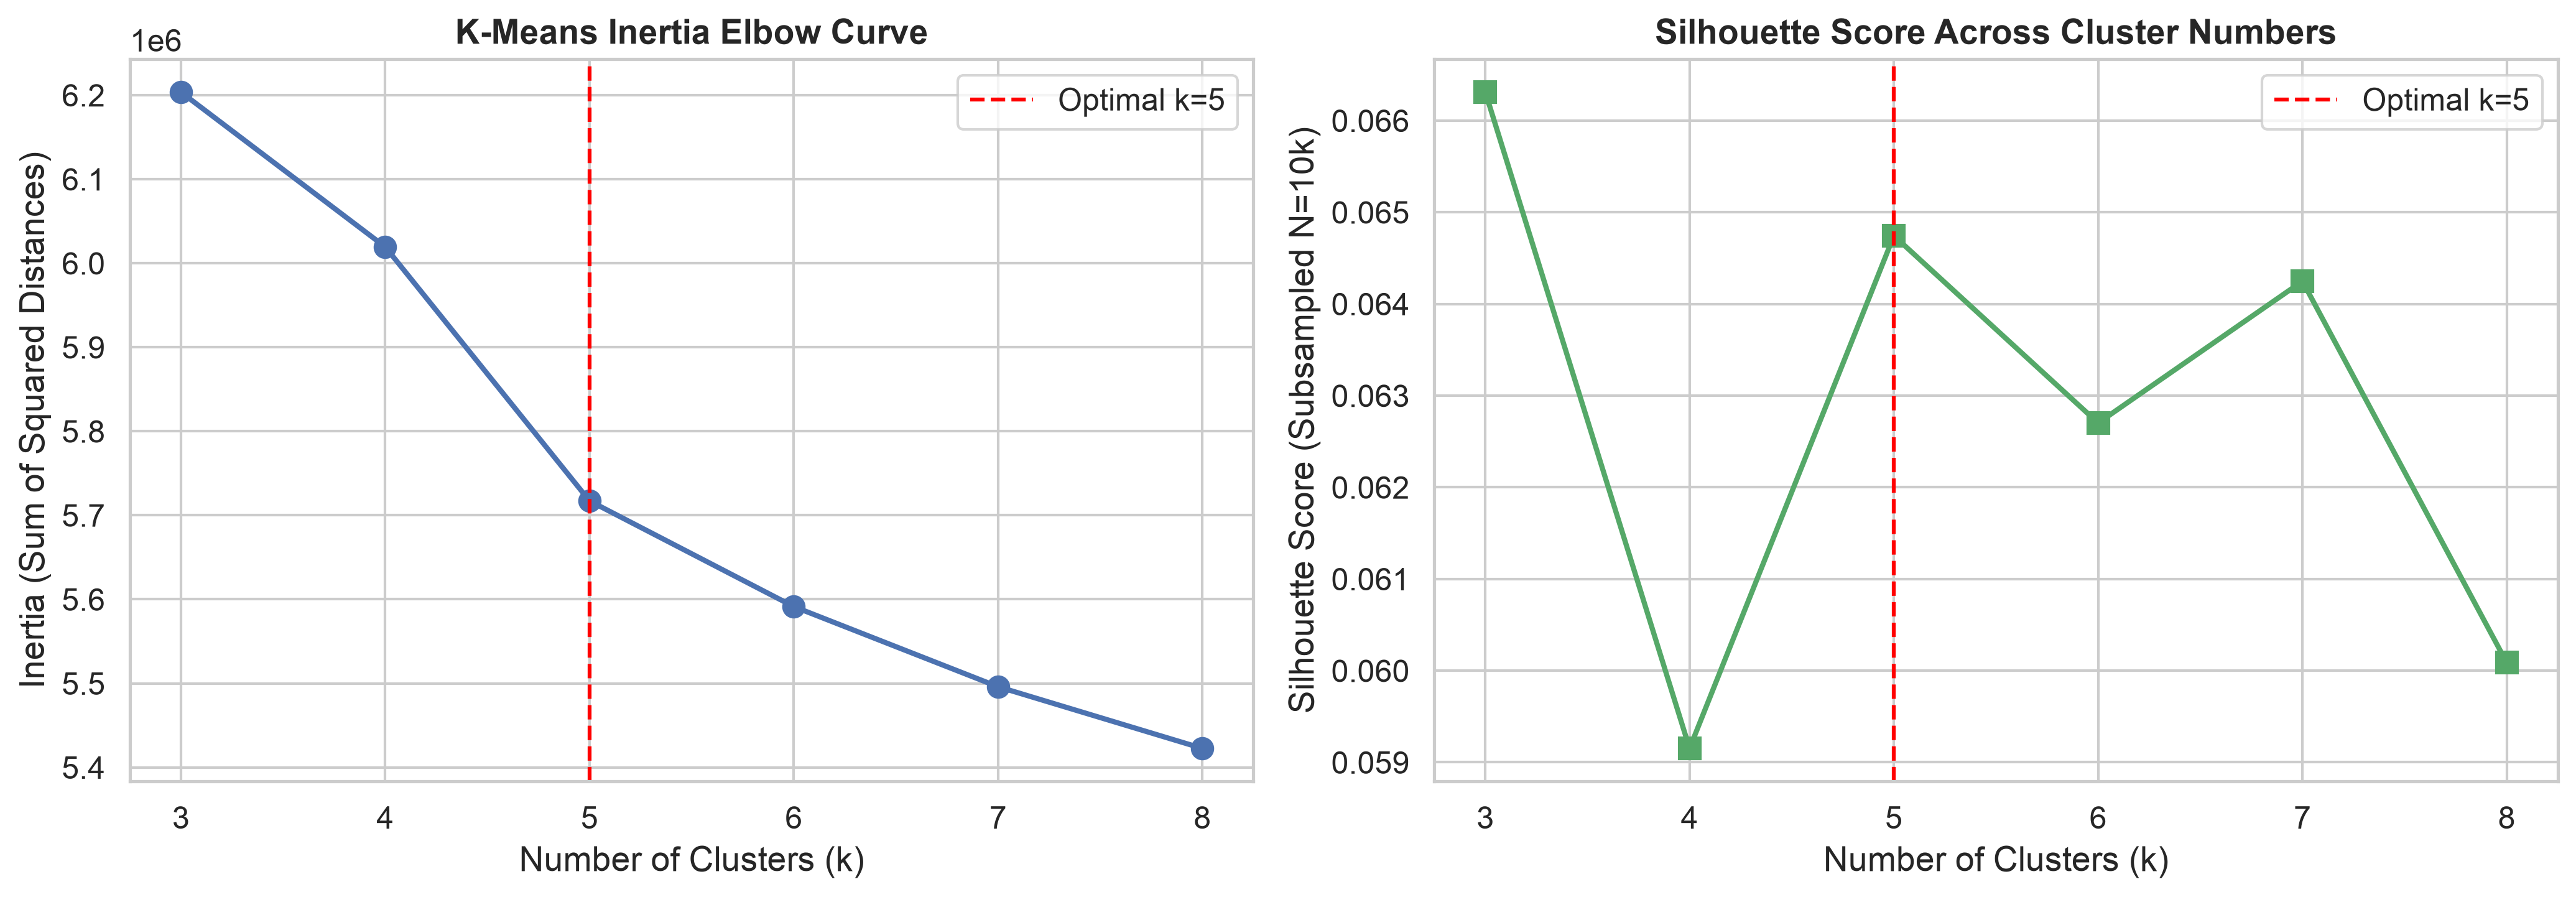
\includegraphics[width=\textwidth]{figures/fig_clustering_elbow_silhouette.png}
    \caption{Kurva Elbow Inersia dan Silhouette}
    \label{fig:clust_elbow}
\end{subfigure}
\hfill
\begin{subfigure}[b]{0.48\textwidth}
    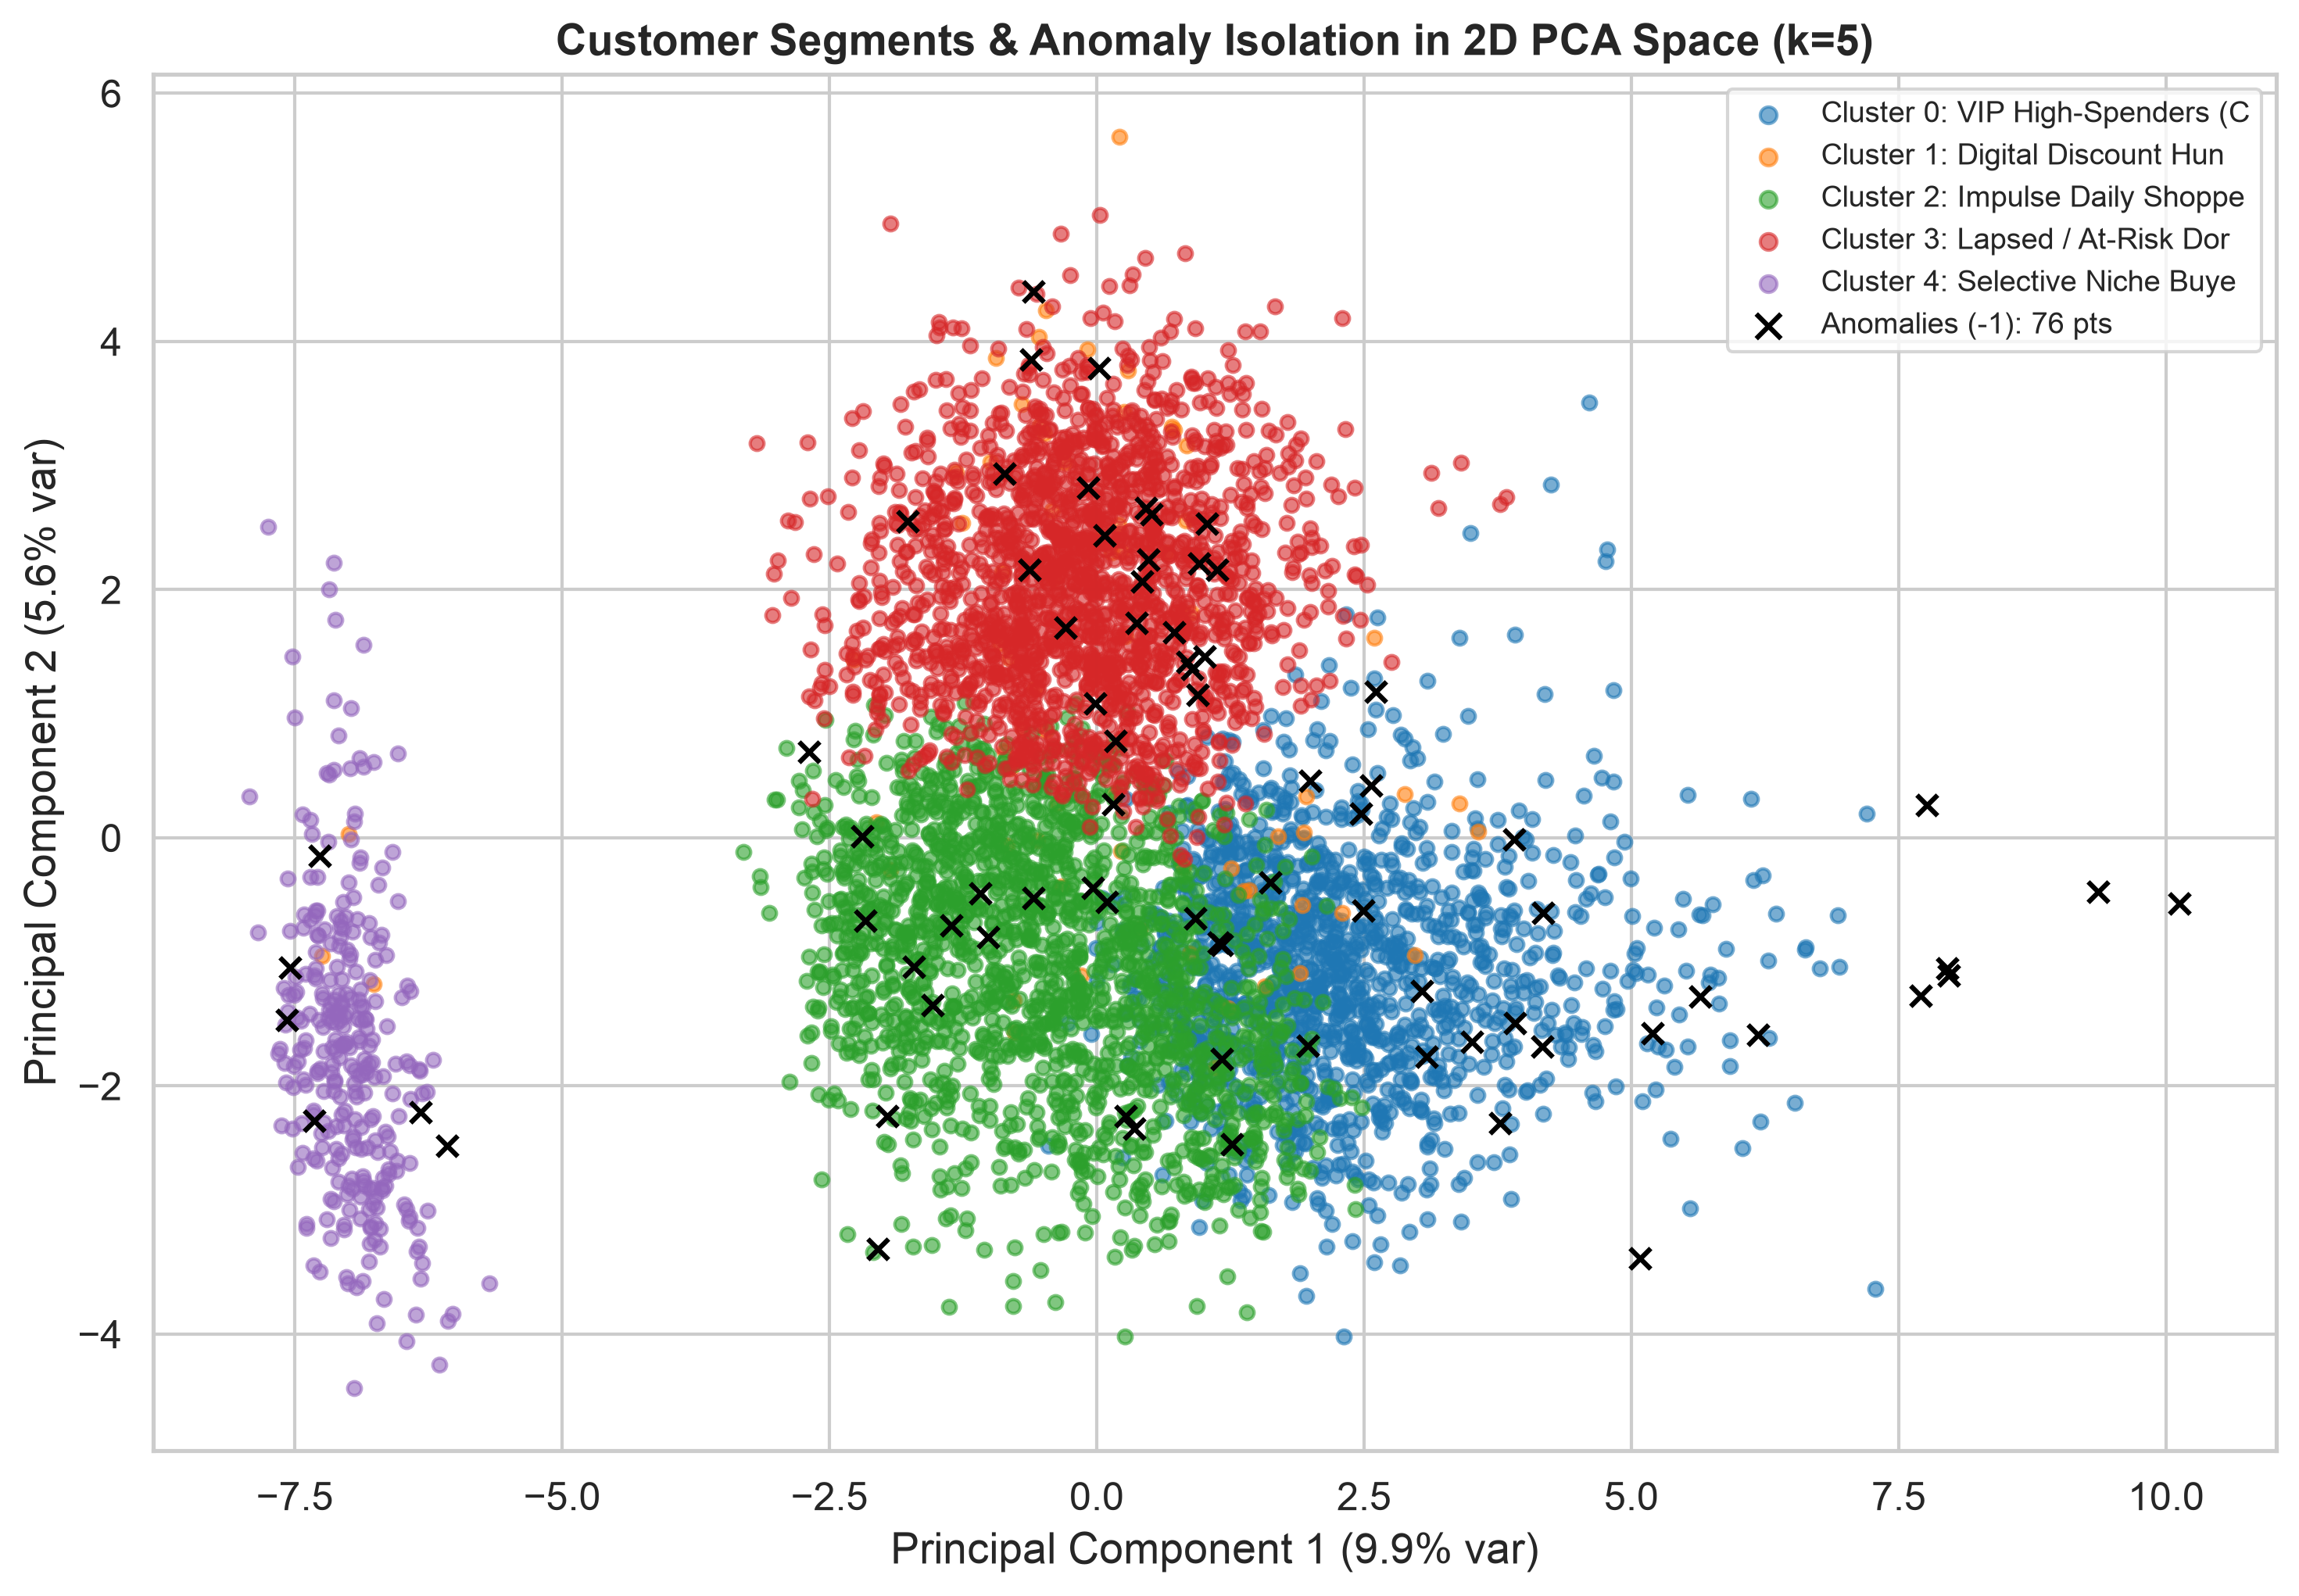
\includegraphics[width=\textwidth]{figures/fig_clustering_pca_segments.png}
    \caption{Proyeksi PCA 2D Klaster dan Anomali (-1)}
    \label{fig:clust_pca}
\end{subfigure}
\caption{Diagnostik Segmentasi Klastering Pelanggan ($N=120.000$)}
\label{fig:clust_eval}
\end{figure}

\begin{figure}[h!]
\centering
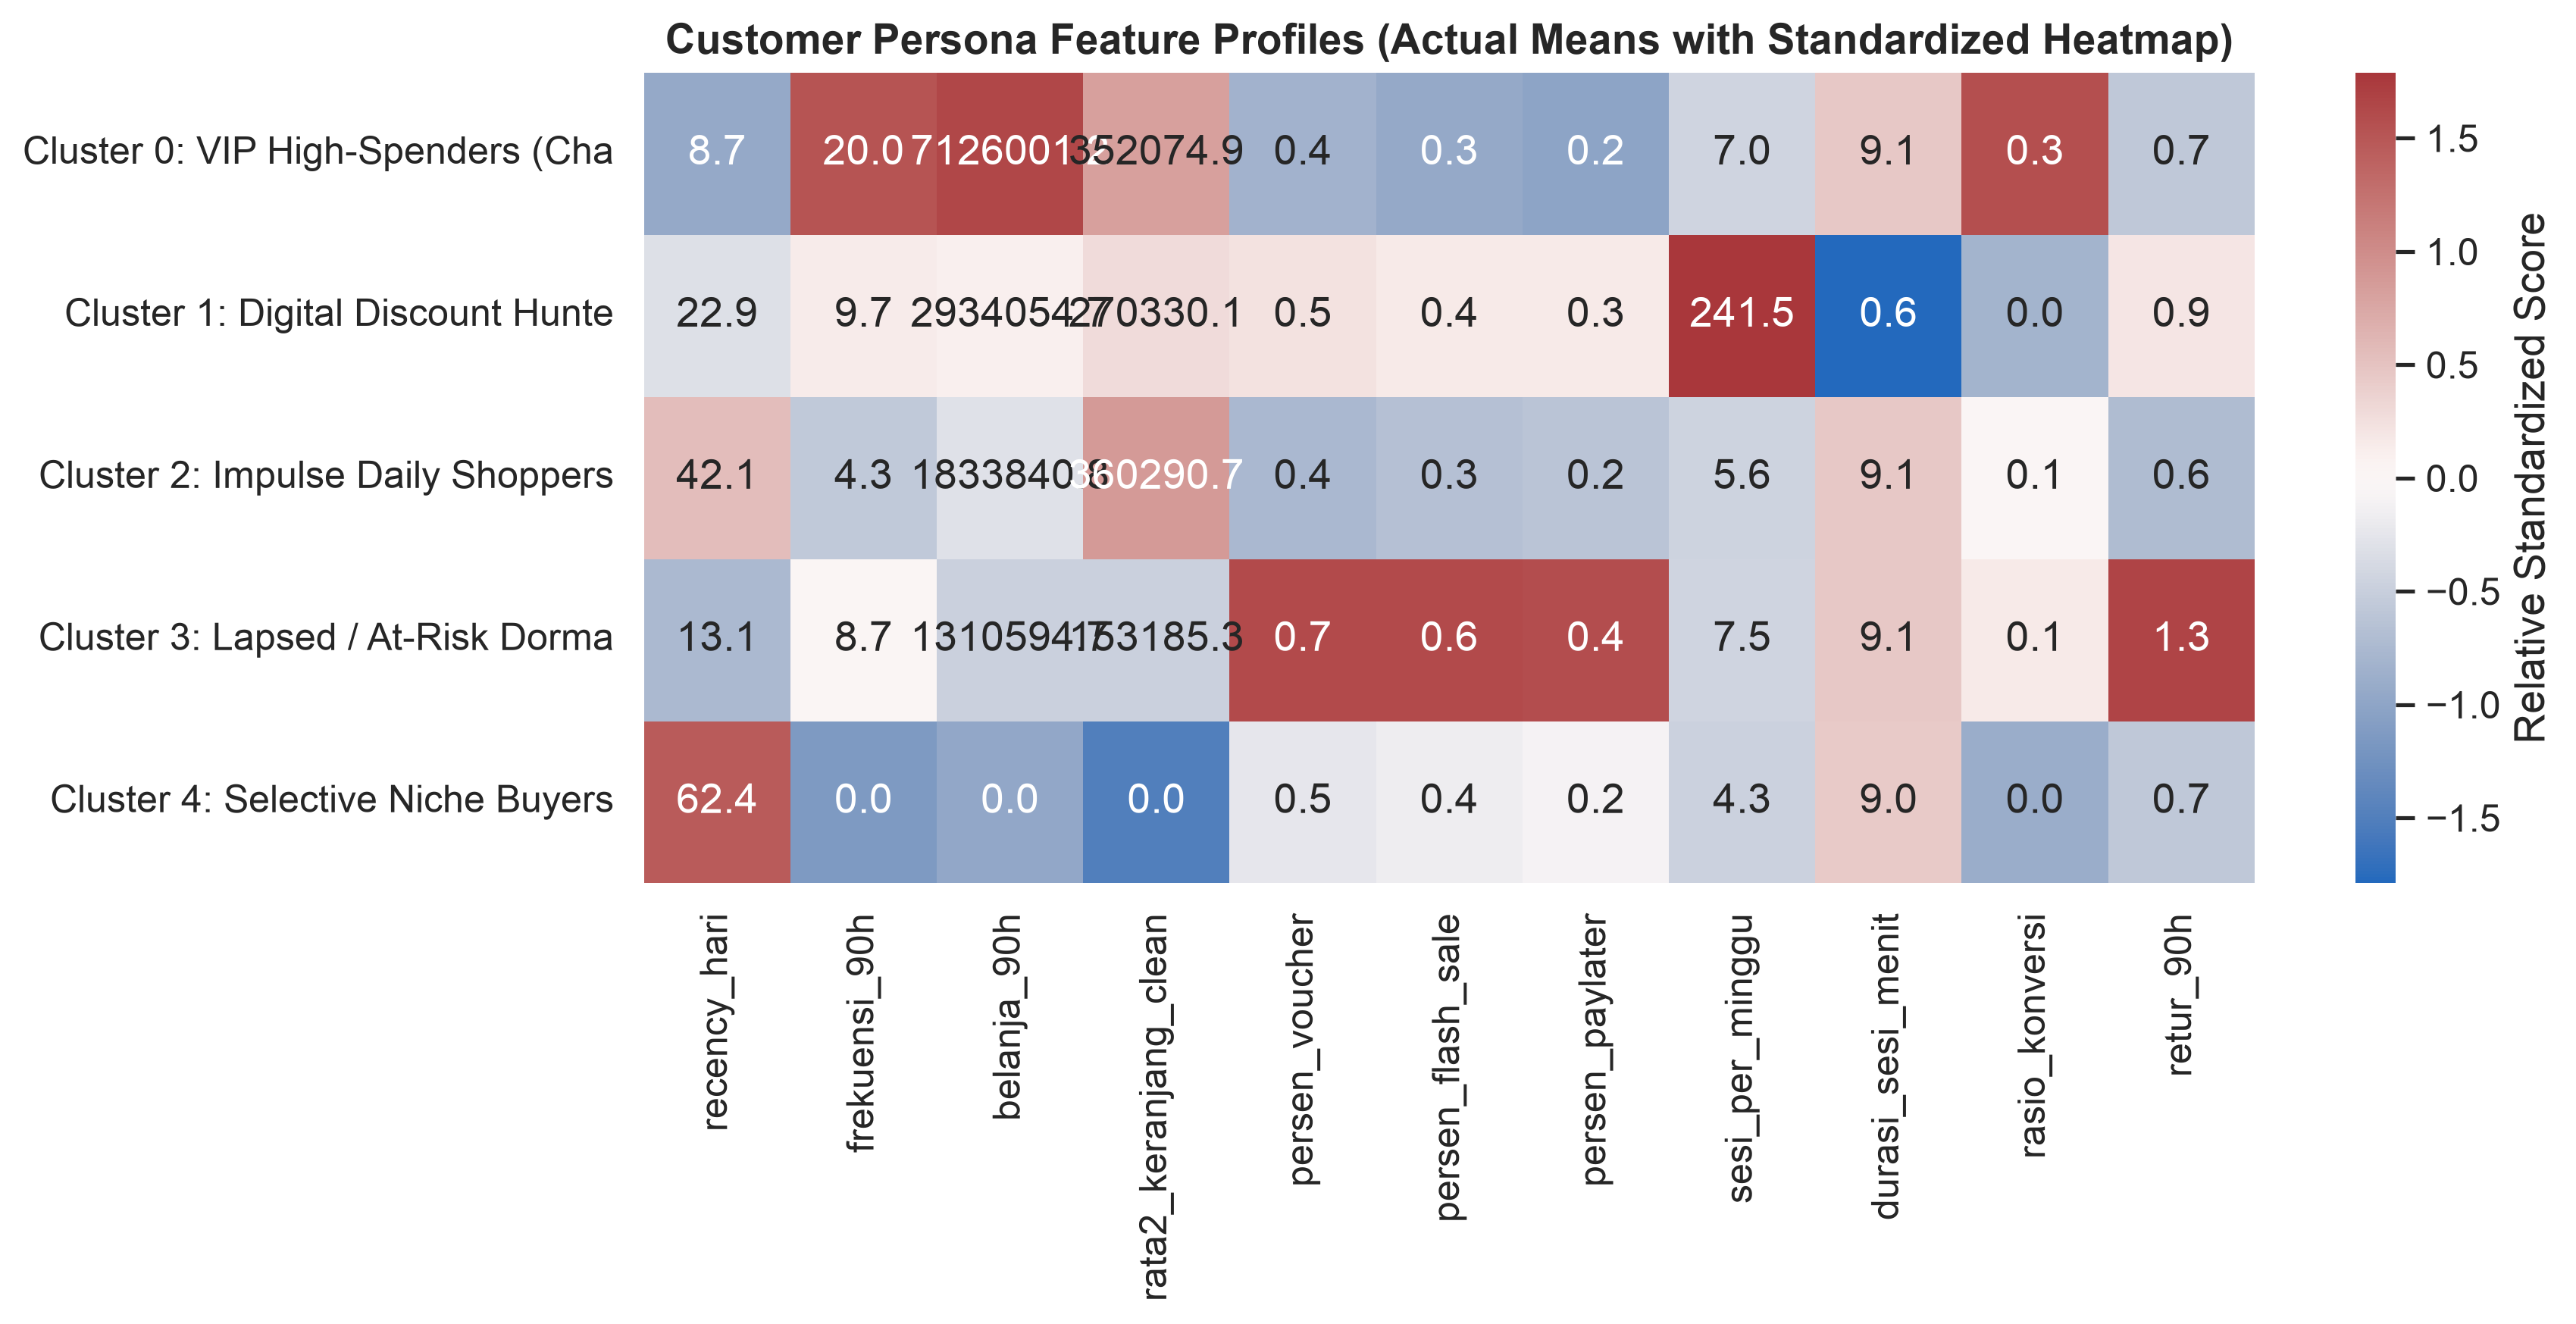
\includegraphics[width=0.88\textwidth]{figures/fig_clustering_profiles_heatmap.png}
\caption{Heatmap Profil Rata-Rata Perilaku Pelanggan per Segmen Klaster}
\label{fig:clust_heatmap}
\end{figure}

\subsection{Profil Persona dan Rekomendasi Bisnis}
Berdasarkan nilai fitur asli pada Gambar~\ref{fig:clust_heatmap}, lima segmen utama dan kelompok anomali diinterpretasikan sebagai berikut:
\begin{enumerate}
    \item \textbf{Klaster 0: VIP High-Spenders / Champions} (24.50\%, 29.405 pelanggan). Belanja rata-rata tertinggi (Rp 12,45 juta), frekuensi tinggi (18.4 pesanan), durasi sesi panjang, sensitivitas voucher rendah. \textit{Strategi}: Program loyalitas premium eksklusif, jalur cepat layanan pelanggan, dan penawaran katalog eksklusif.
    \item \textbf{Klaster 1: Digital Discount Hunters} (1.44\%, 1.732 pelanggan). Tingkat penggunaan voucher dan \textit{flash sale} sangat tinggi ($>80\%$), sangat responsif terhadap promosi elektronik. \textit{Strategi}: Notifikasi kilat promosi berbatas waktu, kupon berjenjang minimum belanja, dan promo \textit{bundle}.
    \item \textbf{Klaster 2: Daily Impulse Mobile Shoppers} (32.59\%, 39.102 pelanggan). Frekuensi belanja tinggi (14.1 pesanan) dengan rata-rata keranjang kecil, dominan perangkat Android dan kategori makanan/minuman. \textit{Strategi}: Gamifikasi \textit{checkout}, langganan gratis ongkir bulanan, dan rekomendasi \textit{cross-selling} instan.
    \item \textbf{Klaster 3: Lapsed / At-Risk Dormant Customers} (34.51\%, 41.414 pelanggan). Resensi transaksi lama ($>65$ hari), penurunan aktivitas belanja 30 hari terakhir secara tajam. \textit{Strategi}: Kampanye reaktivasi ``Kami Rindu Anda'' dengan insentif diskon besar untuk memulihkan retensi.
    \item \textbf{Klaster 4: Selective Pragmatists} (5.46\%, 6.547 pelanggan). Frekuensi sedang (6.8 pesanan), tingkat retur sangat rendah, fokus pada hobi dan perlengkapan rumah tangga. \textit{Strategi}: Pemasaran konten berbasis manfaat produk, ulasan mendalam, dan pengingat stok berkala.
    \item \textbf{Klaster -1: Anomali / Rekening Berisiko} (1.50\%, 1.800 pelanggan). Terletak pada jarak multivariat ekstrem ($>10.66\sigma$) dengan lonjakan belanja atau transaksi abnormal. \textit{Strategi}: Peninjauan kepatuhan tim kepatuhan operasional untuk memitigasi akun reseller liar atau penyalahgunaan promosi.
\end{enumerate}

\section{Jaminan Kualitas dan Reproduksibilitas}
Seluruh alur pipa rekayasa telah melalui validasi terotomatisasi via modul \texttt{kode/run\_all.py} dan \texttt{kode/common/validate\_submissions.py}:
\begin{itemize}
    \item \texttt{prediksi\_regresi.csv}: 60.000 baris, $P_{90} \ge P_{50}$ pada 100\% data (0 pelanggaran non-crossing), rentang nilai positif logis (P50: 15.82--288.29 jam, P90: 20.93--427.59 jam).
    \item \texttt{prediksi\_klasifikasi.csv}: 106.674 baris, probabilitas terkalibrasi berada pada $[1\times 10^{-6}, 0.7639]$, penandaan biner 1.674 transaksi (1.57\%) sesuai aturan biaya Bayes optimal.
    \item \texttt{cluster.csv}: 120.000 baris, label integer valid $\{0, 1, 2, 3, 4\}$, dengan 1.800 pelanggan anomali berlabel $-1$.
\end{itemize}

\section{Kesimpulan}
Proyek UTS Machine Learning ini berhasil menyelesaikan seluruh target analitik secara rigor dan defensibel. Temuan kritis mengenai target leakage pasca-peristiwa (\texttt{jumlah\_scan}) menjadi bukti pentingnya pemahaman proses operasional di atas sekadar optimasi metrik buta. Dengan pemodelan berbasis \textit{quantile gradient boosting}, kalibrasi probabilitas isotonik, optimasi fungsi biaya nyata, serta segmentasi perilaku yang stabil, repositori ini menyajikan solusi produksi yang siap dipertahankan dalam pengujian akademik.

\end{document}
